
\newcommand{\castpatternsection}[1]{\noindent\textbf{#1.}}
\newcommand{\pname}[1]{\textsc{#1}}
\newcommand{\group}[1]{

\

\

{\noindent\Large\textsc{#1} Patterns}

\

\begin{figure}[ht!]
\centering
\includegraphics[width=\textwidth]{"analysis/table-patterns-5000-by-group-#1"}
\caption{#1 Cast Pattern Occurrences}
\label{fig:group-patterns:#1}
\end{figure}

}

\newenvironment{pattern}[1]{
	\newcommand{\desc}{\castpatternsection{Description}}
	\newcommand{\instances}{\castpatternsection{Instances}}
	\newcommand{\detection}{\castpatternsection{Detection}}
	\newcommand{\discussion}{\castpatternsection{Discussion}}
	\newcommand{\related}{\castpatternsection{Related Patterns}}
    \newcommand{\thisp}{\textsc{#1}}
    \subsection{\pname{#1}}
    \label{pat:#1}
	\desc
}{}


\section{Cast Usage Patterns}
\label{sec:casts:patterns}

Using the methodology described in the above section,
we have devised \npattern{} cast usage patterns.
We have excluded casts that represent primitive numeric type conversions,
as they do not represent any pattern.
However, during our manual analysis we found \nprim{} primitive conversions.
Moreover, we found \nbrokenlinks{} links that were not accessible during our analysis.

In this section we present the cast usage patterns we found.
To ease the patterns presentation,
%
\todo{Nate: Overview of categories.}
\todo{Nate: Explain why each pattern belongs to a certain category.}
\todo{Nate: Try to lump together patterns into fewer categories.}
%
we have organized them into \ngroup{} categories according to their purpose.
Table~\ref{table:casts:patterns} presents each pattern and the groups they belong to.
Moreover, we are interested in the scope of the cast instance,
\ie, \emph{does it appear in application source code, test code, or generated code?}
%
\todo{Matthias: Add a paragraph describing and analyzing what one sees in that figure.}
%
Figure~\ref{fig:patterns} shows our patterns and their occurrences sorted by frequency.
The column on the right corresponds to the group the pattern belongs to.
\todo{Describe where patterns come from. Sample -> Invent patterns -> repeat.?}


\begin{table*}[t!]
\scriptsize
\centering
\caption{Patterns and their occurrences in the Maven Central repository.}
\label{table:casts:patterns}
\begin{tabularx}{\linewidth}{rp{2.5cm}llX}
\hdr \# & \textbf{Cast Pattern} & \textbf{Cast Pattern Description} & \textbf{Group} & \textbf{Group Description} \\
\alt  1 & PatternMatching & Cast guarded with an \code{instanceof} operator. & \multirow{4}{*}{Guarded}{Guarded casts.} & \\
\row  2 & TypeTag & \\
\alt  3 & Equals & \\
\row  4 & GetByClassLiteral & \\
\alt  5 & Family & & & \\
\row  6 & Factory & & & \\
\alt  7 & KnownLibraryMethod & & & \\
\row  8 & Tag & & & \\
\alt  9 & Deserialization & & & \\
\row 10 & StackSymbol & & & \\
\alt 11 & CreateByClassLiteral & & & \\
\row 12 & LookupById & & & \\
\alt 13 & StaticResource & & & \\
\row 14 & ObjectAsArray & & & \\
\alt 15 & SelectOverload & & & \\
\row 16 & AccessPrivateField & & & \\
\alt 17 & Clone & & & \\
\row 18 & CovariantReturn & & & \\
\alt 19 & RemoveTypeParameter & & & \\
\row 20 & ImplicitIntersectionType & & & \\
\alt 21 & ImplicitUnionType & & & \\
\row 22 & SoleSubclassImplementation & & & \\
\alt 23 & RecursiveGeneric & & & \\
\row 24 & NewDynamicInstance & & & \\
\alt 25 & ReflectiveAccesibility & & & \\
\row 26 & UncheckedCast & & & \\
\alt 27 & GenericArray & & & \\
\row 28 & RemoveWildcard & & & \\
\alt 29 & Literal & & & \\
\row 30 & RawTypes & & & \\
\alt 31 & Redundant & & & \\
\row 32 & VariableLessSpecificType & & & \\
\hline
\end{tabularx}
\end{table*}





% 'Guarded' = c('PatternMatching', 'TypeTag', "Equals", 'GetByClassLiteral'),
% 'Creational' = c('Family', 'Factory', 'KnownLibraryMethod', 'Tag', 'Deserialization', 'CreateByClassLiteral', 'StackSymbol'),
% 'Tuples' = c('LookupById', 'ObjectAsArray', 'StaticResource'),
% 'Member\nResolution' = c('SelectOverload', 'AccessPrivateField'),
% 'Variance' = c('Clone', 'CovariantReturn', 'RemoveTypeParameter'),
% 'Implicit\nTypes' = c('ImplicitIntersectionType', 'ImplicitUnionType'),
% 'Structural' = c('SoleSubclassImplementation', 'RecursiveGeneric'),
% 'Reflection' = c('ReflectiveAccesibility', 'NewDynamicInstance'),
% 'Unchecked' = c('UncheckedCast', 'RemoveWildcard', 'GenericArray'),
% 'Code Smell' = c('Redundant', 'VariableLessSpecificType', 'RawTypes', 'Literal')


\clearpage

\begin{figure}[ht!]
\centering
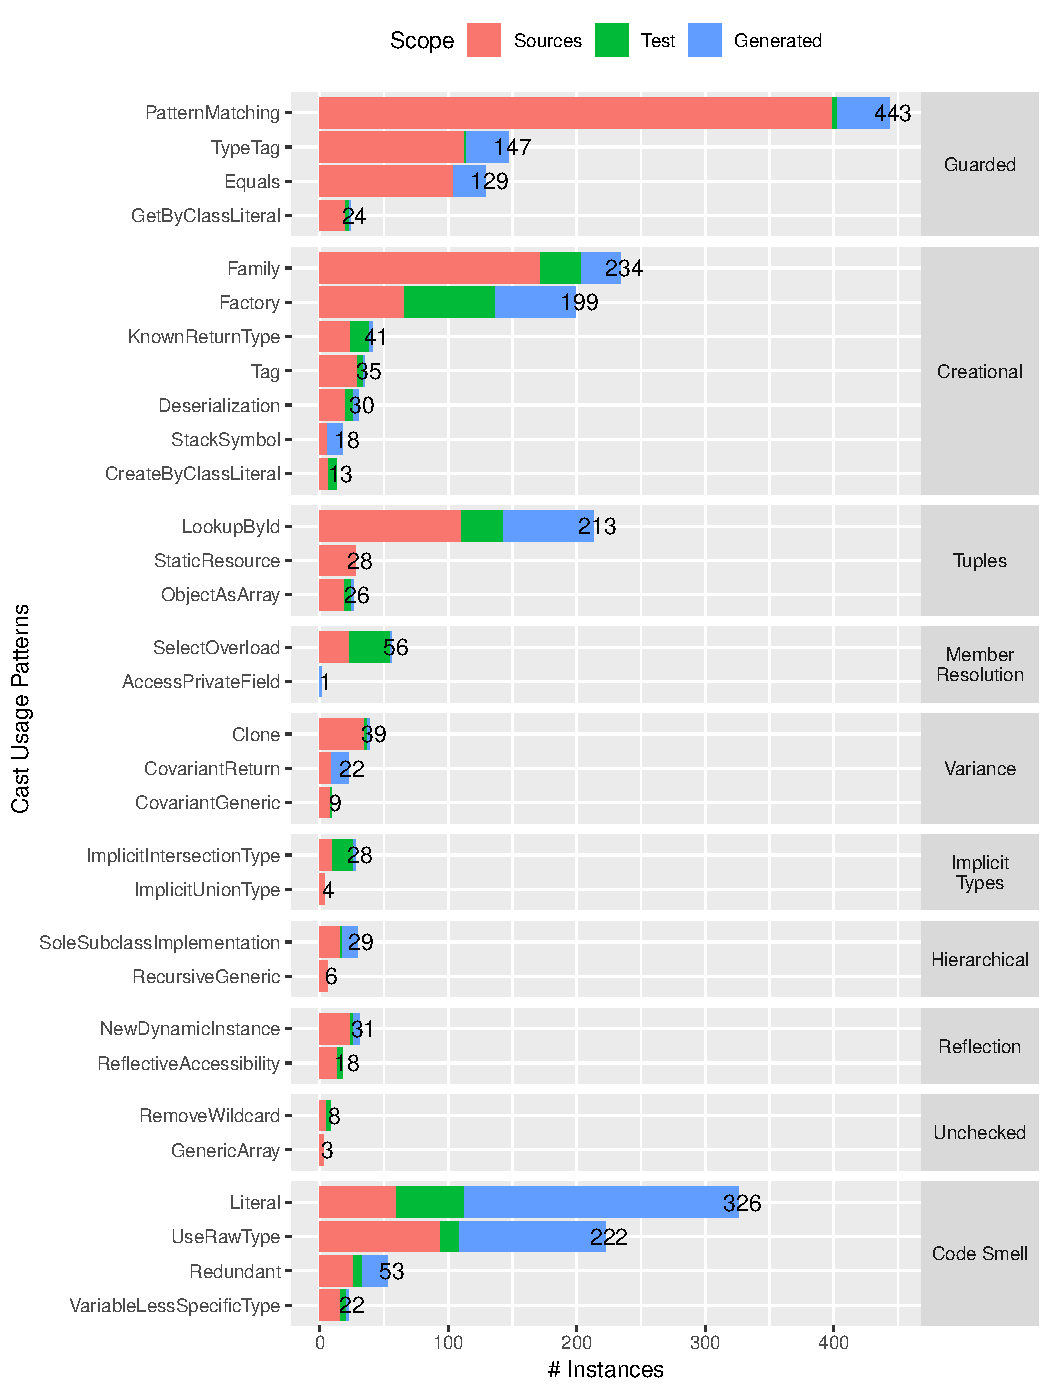
\includegraphics[width=\textwidth]{analysis/table-patterns-5000.pdf}
\caption{Cast Pattern Occurrences} \label{fig:patterns}
\end{figure}

\discuss{Matthias: Start a new subsection here.}
\todo{Matthias: When describing each pattern, you may want to repeat the number of occurrences within the description {\scriptsize (maybe as part of the section title, or just below)}}
Each pattern is described using the following template:

\begin{itemize}
\item \textbf{Description.}
Tells what the pattern is about.
It gives a general overview of the structure of the pattern.
\item \textbf{Instances.}
Gives one or more concrete examples found in real code.
%
\done{Nate: What's the orange (hightlight color) mean? The line with the cast being inspected. Explain here}
%
Each example contains a highlighted line which shows the cast instance being inspected.
Please notice that the snippets presented here were slightly
modified for formatting purposes.
Moreover, to facilitate some snippet presentations,
we remove irrelevant code and replace it with the
comment \code{// [...]}.
For each instance presented here, we provide the link to the source code repository in \lgtm{}.
We provide the link in case the reader wants to do further inspection
of the presented snippet.
%
\done{Nate: List project name too.}
%
Instead of presenting \lgtm{} long URLs,
we have used the URL shortening service
\href{https://bitly.com/}{\bitly} for easier reading.
%
\done{Luis: Links were customized to include the project names.}
%
Each \bitly{} link was customized to include the project name.
\item \textbf{Detection.}
Describes briefly how this pattern was detected in terms of the tags introduced in the previous section.
\item \textbf{Discussion.}
Presents suggestions, flaws, or comments about the pattern.
\item \textbf{Related Patterns.}
%
\done{Nate: Remove "?"}
%
How the pattern being described relates to other patterns.
\end{itemize}

\group{Guarded}

\done{Matthias: Say what it means to be guarded.}
The patterns in this category are guarded casts.
A guarded cast is a cast such that before the cast is applied,
some condition --- the \emph{guard} -- needs to be verified.
The condition to be verified guarantees that the cast will not fail at runtime (unless there is a bug in the application), \ie,
the cast will not throw a \code{ClassCastException}.
Some kind of guards ensure that the cast will not fail at the language-level,
while others only can guarantee it at the application-level.

\begin{pattern}{PatternMatching}
This pattern is composed of a guard (\code{instanceof}) followed by a cast to known subtypes of the static type.
Often there is just one case and the default case, \ie, \code{instanceof} fails, does a no-op or reports an error.
Another common approach is to have several cases,
usually one \emph{per} subtype.

\instances{}
The following listing shows an example of the \thisp{} pattern.%
\footnote{\url{http://bit.ly/OpenMods_OpenBlocks_2FzYYHq}}
%
\done{Nate: Highlightlines color difficult to read}
%
In this example, there is only a single case (line 3).
After the cast is done, a specific operation is performed on the cast type,
\ie, invoking the \code{checkBlock} method.

%https://lgtm.com/projects/g/OpenMods/OpenBlocks/snapshot/dist-2040060754-1524814812150/files/build/sources/java/openblocks/common/tileentity/TileEntityImaginary.java?sort=name&dir=ASC&mode=heatmap#L268
\begin{minted}[highlightlines=3]{java}
Item item = helmet.getItem();
if (item instanceof ItemImaginationGlasses)
	return ((ItemImaginationGlasses)item).checkBlock(what, helmet, this);
\end{minted}

In the next case,%
\footnote{\url{http://bit.ly/PenguinSquad_Enchiridion_2HnNwB7}}
more than one type test are performed.
Each cast corresponds to a type test.

%https://lgtm.com/projects/g/PenguinSquad/Enchiridion/snapshot/dist-19218583-1524814812150/files/build/sources/main/java/joshie/enchiridion/helpers/StackHelper.java?sort=name&dir=ASC&mode=heatmap#L27
\begin{minted}[highlightlines=7]{java}
public static String getStringFromObject(Object object) {
	if (object instanceof Item) {
		return getStringFromStack(new ItemStack((Item) object));
	} else if (object instanceof Block) {
		return getStringFromStack(new ItemStack((Block) object));
	} else if (object instanceof ItemStack) {
		return getStringFromStack((ItemStack) object);
	} else if (object instanceof String) {
		return (String) object;
	} else if (object instanceof List) {
		return getStringFromStack((ItemStack) ((List) object).get(0));
	} else return "";
}
\end{minted}

There are situations when the type test is applied to more than one variable.
In the following example%
\footnote{\url{http://bit.ly/bbossgroups_bboss_2FDN9Rd}}
a double type test is performed on the parameters \code{o1} and \code{o2}.

%https://lgtm.com/projects/g/bbossgroups/bboss/snapshot/dist-2025970729-1524814812150/files/bboss-util/src/org/frameworkset/util/ObjectUtils.java?sort=name&dir=ASC&mode=heatmap#L228
\begin{minted}[highlightlines=25]{java}
public static boolean nullSafeEquals(Object o1, Object o2) {
	if (o1 == o2) {
		return true;
	}
	if (o1 == null || o2 == null) {
		return false;
	}
	if (o1.equals(o2)) {
		return true;
	}
	if (o1.getClass().isArray() && o2.getClass().isArray()) {
		if (o1 instanceof Object[] && o2 instanceof Object[]) {
			return Arrays.equals((Object[]) o1, (Object[]) o2);
		}
		if (o1 instanceof boolean[] && o2 instanceof boolean[]) {
			return Arrays.equals((boolean[]) o1, (boolean[]) o2);
		}
		if (o1 instanceof byte[] && o2 instanceof byte[]) {
			return Arrays.equals((byte[]) o1, (byte[]) o2);
		}
		if (o1 instanceof char[] && o2 instanceof char[]) {
			return Arrays.equals((char[]) o1, (char[]) o2);
		}
		if (o1 instanceof double[] && o2 instanceof double[]) {
			return Arrays.equals((double[]) o1, (double[]) o2);
		}
		if (o1 instanceof float[] && o2 instanceof float[]) {
			return Arrays.equals((float[]) o1, (float[]) o2);
		}
		if (o1 instanceof int[] && o2 instanceof int[]) {
			return Arrays.equals((int[]) o1, (int[]) o2);
		}
		if (o1 instanceof long[] && o2 instanceof long[]) {
			return Arrays.equals((long[]) o1, (long[]) o2);
		}
		if (o1 instanceof short[] && o2 instanceof short[]) {
			return Arrays.equals((short[]) o1, (short[]) o2);
		}
	}
	return false;
}
\end{minted}

Another common scenario%
\footnote{\url{http://bit.ly/codefollower_Tomcat-Research_2SGDUG5}}
is when several cases are used to re-\code{throw} an exception of the right type, as shown below.
The cast instance is applied to a variable of type \code{Throwable}
(line 13).
Nevertheless, the enclosing method is only allowed to throw \code{NamingException} by the \code{throws} declaration (line 3).
Since an exception of type \code{Throwable} is checked,
a cast to \code{VirtualMachineError} (subclass of \code{Error}) is needed.

%https://lgtm.com/projects/g/codefollower/Tomcat-Research/snapshot/dist-13734061-1524814812150/files/java/org/apache/naming/factory/DataSourceLinkFactory.java?sort=name&dir=ASC&mode=heatmap#L85
\begin{minted}[highlightlines=13]{java}
protected Object wrapDataSource(
			Object datasource, String username, String password)
			throws NamingException {
	try {
		// [...]
	}catch (Exception x) {
		if (x instanceof InvocationTargetException) {
			Throwable cause = x.getCause();
			if (cause instanceof ThreadDeath) {
				throw (ThreadDeath) cause;
			}
			if (cause instanceof VirtualMachineError) {
				throw (VirtualMachineError) cause;
			}
			if (cause instanceof Exception) {
				x = (Exception) cause;
			}
		}
		if (x instanceof NamingException) throw (NamingException)x;
		else {
			// [...]
		}
	}
}
\end{minted}

The next example%
\footnote{\url{http://bit.ly/kiegroup_jbpm_2ENCL8a}}
shows how \thisp{} can be used to filter elements by type within a stream.
The cast instance is applied to stream operations (line 3) over the \code{caseAssignments} collection.
The filter operation by type is performed in line 4.

%https://lgtm.com/projects/g/kiegroup/jbpm/snapshot/dist-1810050-1524814812150/files/jbpm-case-mgmt/jbpm-case-mgmt-impl/src/main/java/org/jbpm/casemgmt/impl/wih/StartCaseWorkItemHandler.java?sort=name&dir=ASC&mode=heatmap#L212
\begin{minted}[highlightlines=3]{java}
Collection<OrganizationalEntity> caseAssignments = 
		((CaseAssignment)caseFile).getAssignments(name);
user = (User) caseAssignments.stream()
		.filter(oe -> oe instanceof User)
		.findFirst()
		.orElseThrow(() -> new IllegalArgumentException());

public interface User extends OrganizationalEntity {}
public interface OrganizationalEntity {}
\end{minted}


\detection{}
To detect this pattern,
a cast needs to be guarded by an \code{instanceof} expression.
The operand expression to both the cast and the \code{instanceof} needs to be the same.
In the case the operand expression is a variable, we also check that there is no assignment between the \code{instanceof} guard and the cast to that variable.

In some situations, the operand expression is a method invocation.
%
\done{Nate: Avoid "we"}
%
To be an instance of the \thisp{} pattern,
the value returned by the method needs to be the same for both the \code{instanceof} and the cast, \ie, it is a pure method.

\discussion{}
The \thisp{} pattern consists of testing the runtime type of a variable against several related types.
It is a technique that allows a developer to take different actions according to the runtime type of an object.
Depending on the --- runtime --- type of an object, different cases, usually one for each type will follow.

The \thisp{} pattern can be seen as an \adhoc{} alternative to pattern matching as a language construct~\citep{lavilleLazyPatternMatching1987}.
This construct can be seen in several other languages, \eg, \scala{}, \csharp{}, and \haskell{}.
For instance, in \scala{} the pattern matching construct is achieved using the \code{match} keyword.
In this example,%
\footnote{Adapted from \url{https://docs.scala-lang.org/tour/pattern-matching.html}}
a different action is taken according to the runtime type of the parameter \code{notification} (line 9).

\begin{minted}[highlightlines=10]{scala}
abstract class Notification
case class Email(sender: String, title: String, body: String)
	extends Notification
case class SMS(caller: String, message: String)
	extends Notification
case class VoiceRecording(contactName: String, link: String)
	extends Notification

def showNotification(notification: Notification): String = {
	notification match {
		case Email(email, title, _) =>
		s"You got an email from $email with title: $title"
		case SMS(number, message) =>
		s"You got an SMS from $number! Message: $message"
		case VoiceRecording(name, link) =>
		s"Voice Recording from $name! Click the link: $link"
	}
	}
	val someSms = SMS("12345", "Are you there?")
	val someVoiceRecording = VoiceRecording("Tom", "voicerecording.org/id/123")
	
	// prints You got an SMS from 12345! Message: Are you there?
	println(showNotification(someSms))
	
	// Voice Recording from Tom! Click the link: voicerecording.org/id/123	
	println(showNotification(someVoiceRecording))
\end{minted}

As a workaround, alternatives to the \thisp{} pattern can be the visitor pattern or polymorphism.
But in some cases, the chain of \code{instanceof}s is of boxed types.
Thus no polymorphism can be used.
There is an ongoing proposal%
\footnote{\url{http://openjdk.java.net/jeps/305}}$^{,}$%
\footnote{\url{https://cr.openjdk.java.net/~briangoetz/amber/pattern-match.html}}
to add pattern matching to the \java{} language.
The proposal explores how to change the \code{instanceof} operator in order to support pattern matching.
%
\done{Java 12 will (maybe) add matching.}
%
\java{} 12 already extends the \code{switch} statement to be used as either a statement or an expression.%
\footnote{\url{https://openjdk.java.net/jeps/325}}
This enhancement aims to ease the transition to a \code{switch} expression that supports pattern matching.

\related{}
The \nameref{pat:Equals} pattern can be seen as a special case of the \thisp{} pattern,
because often the parameter to the \code{equals} method is guarded by an \code{instanceof} expression.
\end{pattern}

\begin{pattern}{Equals}
This pattern is a common pattern to implement the well-known \code{equals} method (declared in \code{java.lang.Object}).
It is a particularly instance of guarded casts.
A cast expression is guarded by either an
\code{instanceof} test---\variant{InstanceOf} variant---or a
\code{getClass} comparison---\variant{GetClass} variant---usually to the same target type as the cast;
in an \code{equals}%
\footnote{\url{https://docs.oracle.com/javase/8/docs/api/java/lang/Object.html\#equals-java.lang.Object-}}
method implementation.
This is done to check if the argument has same type as the receiver
(\code{this} argument).
Notice that a cast in an \code{equals} method is needed because it
receives an \code{Object} as a parameter.

To detect this pattern,
a cast must be applied to the parameter of the \code{equals} method.
The result value of the cast must be then used in an equality comparison.
We relax the constraint that the target type of the cast must the enclosing class.

\instances{}
This pattern accounts for \nEqualsOutofGuarded\% of guarded casts,
\nEqualsPattern{} instances out of \nGuarded{}.
Figure~\ref{fig:casts:equals} shows the different variants of the \thisp{} pattern and their occurrences.
The \variant{InstanceOfSupertype}, \variant{AutoValue}, and
\variant{InstanceOfSwitch} variants are explained below.

\plot{patterns/table-pattern-Equals-Equals-args}{fig:casts:equals}{\thisp{} Variants Occurrences}

The following listing shows an example of the \thisp{} pattern.
In this case,
\code{instanceof} is used to guard for the same type as the receiver 
(\variant{InstanceOf} variant).

%https://lgtm.com/projects/g/neo4j/neo4j/snapshot/dist-15760049-1519892555006/files/community/kernel/src/main/java/org/neo4j/kernel/impl/api/CountsRecordState.java?sort=name&dir=ASC&mode=heatmap&excluded=false#L182
\def\urlvar{http://bit.ly/neo4j_neo4j_2vJw94J}
\begin{minted}[highlightlines=7]{java}
@Override
public boolean equals(Object obj) {
    if ( this == obj ) {
        return true;
    }
    if ( (obj instanceof Difference) ) {
        Difference that = (Difference) obj;
        return actualFirst == that.actualFirst
          && expectedFirst == that.expectedFirst
          && actualSecond == that.actualSecond 
          && expectedSecond == that.expectedSecond
          && key.equals( that.key );
    }
    return false;
} #\urlbox#
\end{minted}

Alternatively, the following listing shows another example of the \thisp{} pattern.
But in this case,
a \code{getClass} comparison is used to guard for the same type as the receiver in line 4 (\variant{GetClass} variant).

%https://lgtm.com/projects/g/neo4j/neo4j/snapshot/dist-15760049-1519892555006/files/community/bolt/src/main/java/org/neo4j/bolt/v1/messaging/infrastructure/ValuePath.java?sort=name&dir=ASC&mode=heatmap&excluded=false#L278
\def\urlvar{http://bit.ly/neo4j_neo4j_2vKP0MW}
\begin{minted}[highlightlines=7]{java}
@Override
public boolean equals( Object o ) {
    if ( this == o ) return true;
    if ( o == null || getClass() != o.getClass() )
        return false;

    ValuePath that = (ValuePath) o;
    return nodes.equals(that.nodes) &&
        relationships.equals(that.relationships);
} #\urlbox#
\end{minted}

In some situations, the type cast is not the same as the enclosing class.
Instead, the target type of the cast is the super class or a super interface of the enclosing class (\variant{InstanceOfSupertype} variant).
The following example shows this scenario.
The cast is performed in the \code{WildcardTypeImpl} enclosing class,
but the target type is \code{java.lang.reflect.WildcardType}.

%https://lgtm.com/projects/g/elastic/elasticsearch/snapshot/dist-1916470085-1524814812150/files/server/src/main/java/org/elasticsearch/common/inject/internal/MoreTypes.java?sort=name&dir=ASC&mode=heatmap#L606
\def\urlvar{http://bit.ly/elastic_elasticsearch_2GHyPp5}
\begin{minted}[highlightlines=5]{java}
public static class WildcardTypeImpl implements WildcardType, CompositeType {
    @Override
    public boolean equals(Object other) {
        return other instanceof WildcardType
                && MoreTypes.equals(this, (WildcardType) other);
    }
} #\urlbox#
\end{minted}

Similar to the previous example, 
the \variant{AutoValue} variant casts the \code{equals} parameter to a super class of the enclosing class.
However, this happens when the Google AutoValue library%
\footnote{\url{https://github.com/google/auto/tree/master/value}}
is used.
AutoValue is a code generator for value classes.

%https://lgtm.com/projects/g/square/sqlbrite/snapshot/3a9916985485ba5922097fe59a18230500f02df4/files/sample/build/generated/source/apt/debug/com/example/sqlbrite/todo/ui/$AutoValue_ListsItem.java?sort=name&dir=ASC&mode=heatmap&showExcluded=false#L52
\def\urlvar{http://bit.ly/square_sqlbrite_2HmHMYE}
\begin{minted}[highlightlines=13]{java}
@AutoValue
abstract class ListsItem implements Parcelable {
    // [...]
}

abstract class $AutoValue_ListsItem extends ListsItem {
    @Override
    public boolean equals(Object o) {
      if (o == this) {
        return true;
      }
      if (o instanceof ListsItem) {
        ListsItem that = (ListsItem) o;
        return (this.id == that.id())
             && (this.name.equals(that.name()))
             && (this.itemCount == that.itemCount());
      }
      return false;
    }
} #\urlbox#
\end{minted}

The following snippet shows a non-trivial implementation of \code{equals}.
The enclosing class of the \code{equals} method is \code{CapReq} (line 1).
However, the cast instance (line 13) is not against the enclosing class,
it is against to the \code{Requirement} class (\variant{InstanceOfSwitch} variant).
Note that the cast using the enclosing class as target type is in line 9.

%https://lgtm.com/projects/g/bndtools/bnd/snapshot/dist-930051-1524814812150/files/biz.aQute.bndlib/src/aQute/bnd/osgi/resource/CapReq.java?sort=name&dir=ASC&mode=heatmap#L73
\def\urlvar{http://bit.ly/bndtools_bnd_2SM5pOw}
\begin{minted}[highlightlines=13]{java}
class CapReq {
    @Override
    public boolean equals(Object obj) {
        if (this == obj)
                return true;
        if (obj == null)
                return false;
        if (obj instanceof CapReq)
                return equalsNative((CapReq) obj);
        if ((mode == MODE.Capability) && (obj instanceof Capability))
                return equalsCap((Capability) obj);
        if ((mode == MODE.Requirement) && (obj instanceof Requirement))
                return equalsReq((Requirement) obj);
        return false;
    }
} #\urlbox#
\end{minted}


\issues{}
The pattern for an \code{equals} method implementation is well-known.
Most \code{equals} methods in our sample are implemented with the same boilerplate structure:
that is, first checking if the parameter is another reference to \code{this},
then checking if the argument is not null,
and finally, checking if the argument is of the right class
(with either an \code{instanceof} test or a \code{getClass} comparison).
Once all checks are performed, a cast follows, and a field-by-field comparison is made.

To avoid this boilerplate, other languages bake in deep equality comparisons,
at least for some types (\eg, \scala{} case classes),
or provide mechanisms to generate the boilerplate code (\eg, \code{deriving Eq}
in \haskell{} or \code{\#[derive(Eq)]} in \rust{}).
\cite{vaziriDeclarativeObjectIdentity2007} propose a declarative approach to avoid boilerplate code when implementing
both the \code{equals} and \code{hashCode} methods.
They manually analyzed several applications, and found there are many issues while implementing \code{equals()} and \code{hashCode()} methods.
It would be interesting to check whether these issues happen in real application code.

There is an exploratory document%
\footnote{\url{http://cr.openjdk.java.net/\~briangoetz/amber/datum.html}}
by Brian Goetz---\java{} Language Architect---addressing these issues from a more general perspective.
It is definitely a starting point towards improving the \java{} language.

This pattern can be seen as a special instance of the \nameref{pat:Typecase} pattern when the guard is an \code{instanceof} test or a \code{getClass} comparison.

\end{pattern}
\begin{pattern}{TypeTag}
%
\done{Matthias: Your first example doesn't have the tag in the *same* object, but passes it as a separate variable.}
%
A cast instance belonging to the \thisp{} pattern is guarded by an application-specific test instead of using an \code{instanceof} test.

\instances{}
The following example%
\footnote{\url{http://bit.ly/JesusFreke_smali_2Ho8bVL}}
shows an instance of the \thisp{} pattern.
The cast type of the parameter \code{reference} is determined by the value of the parameter \code{referenceType}.

%https://lgtm.com/projects/b/JesusFreke/smali/snapshot/dist-1306230039-1524814812150/files/dexlib2/src/main/java/org/jf/dexlib2/writer/InstructionWriter.java?sort=name&dir=ASC&mode=heatmap#L492
\begin{minted}[highlightlines=8]{java}
private int getReferenceIndex(int referenceType, Reference reference) {
    switch (referenceType) {
        case ReferenceType.FIELD:
            return fieldSection.getItemIndex((FieldRefKey) reference);
        case ReferenceType.METHOD:
            return methodSection.getItemIndex((MethodRefKey) reference);
        case ReferenceType.STRING:
            return stringSection.getItemIndex((StringRef) reference);
        case ReferenceType.TYPE:
            return typeSection.getItemIndex((TypeRef) reference);
        case ReferenceType.METHOD_PROTO:
            return protoSection.getItemIndex((ProtoRefKey) reference);
        default:
            throw new ExceptionWithContext(
                "Unknown reference type: %d",  referenceType);
    }
}
\end{minted}

In the next example,%
\footnote{\url{http://bit.ly/FenixEdu_fenixedu-academic_2SUNOUJ}}
instead of a \code{switch} statement,
an \code{if} statement is used to guard the cast (in line 6).

%https://lgtm.com/projects/g/FenixEdu/fenixedu-academic/snapshot/dist-29270029-1524814812150/files/src/main/java/org/fenixedu/academic/ui/renderers/student/curriculum/StudentCurricularPlanRenderer.java?sort=name&dir=ASC&mode=heatmap#L853
\begin{minted}[highlightlines=6]{java}
for (final IEnrolment enrolment : dismissal.getSourceIEnrolments()) {
    if (enrolment.isExternalEnrolment()) {
        generateExternalEnrolmentRow(mainTable, (ExternalEnrolment) enrolment,
                level + 1, true);
    } else {
        generateEnrolmentRow(mainTable, (Enrolment) enrolment,
                level + 1, false, true, true);
    }
}
\end{minted}

\done{Nate: Why is this not pattern matching?}
%
In the next case%
\footnote{\url{http://bit.ly/apache_poi_2FW5SXU}}
a type test is performed --- through a method call --- before actually applying the cast to the variable \code{props} (line 3).
Note that the type test is internally using the \code{instanceof} operator (line 8).
Although in this case the type test is using an \code{instanceof} operator,
it is not considered \nameref{pat:PatternMatching} because the \code{instanceof} is located in a method call.

%https://lgtm.com/projects/g/apache/poi/snapshot/dist-1790760597-1524814812150/files/src/ooxml/java/org/apache/poi/xslf/usermodel/XSLFPropertiesDelegate.java?sort=name&dir=ASC&mode=heatmap#L1367
\begin{minted}[highlightlines=3]{java}
@Override
public CTSolidColorFillProperties getSolidFill() {
    return isSetSolidFill() ? (CTSolidColorFillProperties)props : null;
}

@Override
public boolean isSetSolidFill() {
    return (props instanceof CTSolidColorFillProperties);
}
\end{minted}

In some cases, the type to be cast is the same in every branch.
The following snippet%
\footnote{\url{http://bit.ly/loopj_android-async-http_2IpIULk}}
shows an instance of this case.
The cast is applied to the \code{message.obj} field to (line 13),
according to the value of the \code{message.what} field (line 1).
However, a similar cast is applied in the first branch (line 3).
In both branches \code{message.obj} is of type \code{Object[]},
but in the case of \code{FAILURE\_MESSAGE},
the array contains one more element (line 16).
This suggests that the \code{(Object[]) message.obj} array denotes two different objects,
but are not distinguishable from the type system perspective.

%https://lgtm.com/projects/g/loopj/android-async-http/snapshot/dist-1879340034-1549372228293/files/library/src/main/java/com/loopj/android/http/AsyncHttpResponseHandler.java?sort=name&dir=ASC&mode=heatmap#L359
\begin{minted}[highlightlines=13]{java}
switch (message.what) {
    case SUCCESS_MESSAGE:
        response = (Object[]) message.obj;
        if (response != null && response.length >= 3) {
            onSuccess((Integer) response[0], (Header[]) response[1],
                    (byte[]) response[2]);
        } else {
            AsyncHttpClient.log.e(LOG_TAG, 
                    "SUCCESS_MESSAGE didn't got enough params");
        }
        break;
    case FAILURE_MESSAGE:
        response = (Object[]) message.obj;
        if (response != null && response.length >= 4) {
            onFailure((Integer) response[0], (Header[]) response[1],
                    (byte[]) response[2], (Throwable) response[3]);
        } else {
            AsyncHttpClient.log.e(LOG_TAG,
                    "FAILURE_MESSAGE didn't got enough params");
        }
        break;
    // [...]
}
\end{minted}

In the next example,%
\footnote{\url{http://bit.ly/groovy_groovy-core_2SGzK16}}
the parameter \code{args} is cast to \code{Object[]} (line 13).
The ``type tag'' is given by the fact that the cast is executed in a \code{catch} block,
and that \code{value} is an instance of \code{Closure} (line 9).
The \code{args} parameter flows into two methods,
\code{invokeMethod(String name, Object args)}
and
\code{call(Object... args)}%
.
Thus, \code{args} is treated as an \code{Object} or \code{Object[]} depending on the type tag,
resembling an union type.

%https://lgtm.com/projects/g/groovy/groovy-core/snapshot/dist-45390050-1524814812150/files/src/main/groovy/util/Expando.java?sort=name&dir=ASC&mode=heatmap#L103
\begin{minted}[highlightlines=13]{java}
public Object invokeMethod(String name, Object args) {
    try {
        return super.invokeMethod(name, args);
    }
    catch (GroovyRuntimeException e) {
        // br should get a "native" property match first.
        // getProperty includes such fall-back logic
        Object value = this.getProperty(name);
        if (value instanceof Closure) {
            Closure closure = (Closure) value;
            closure = (Closure) closure.clone();
            closure.setDelegate(this);
            return closure.call((Object[]) args);
        } else {
            throw e;
        }
    }
}
\end{minted}


\detection{}
The detection of this pattern is similar to the \nameref{pat:PatternMatching} detection, but instead of looking for an \code{instanceof} guarded cast, we look for an application-specific guard.
The guard needs to determine either the resulting type of the cast instance, or
the subsequent operations applied to the result of the cast instance if the types in every branch are the same.

\discussion{}
In some cases, the \thisp{} pattern can be replaced by \nameref{pat:PatternMatching}.
However, if the application-specific tag is a numeric value,
the \thisp{} could perform better than the \nameref{pat:PatternMatching} using \code{instanceof}.
Moreover, there are situation where the \thisp{} can not be avoid since the types to be cast are the same.

\related{}
%
\done{Nate: PatternMatching}
This pattern is related to \nameref{pat:PatternMatching} since both denoted guarded casts.
The difference is that \thisp{} uses an application-specific test.
\nameref{pat:GetByClassLiteral} could be seen as a special case of \thisp{} where the tag is a class literal.

\end{pattern}
\begin{pattern}{GetByClassLiteral}
A cast is using an application-specific guard,
but the guard depends on a class literal.

\instances{}
The following example%
\footnote{\url{http://bit.ly/elastic_elasticsearch_2SSgsFV}}
shows an instance of the \thisp{} pattern.
A cast is performed to the \code{field} variable (line 22),
based whether the runtime class of the variable is actually \code{Short.class}.

%https://lgtm.com/projects/g/elastic/elasticsearch/snapshot/dist-1916470085-1524814812150/files/server/src/main/java/org/elasticsearch/common/lucene/Lucene.java?sort=name&dir=ASC&mode=heatmap#L478
\begin{minted}[highlightlines=22]{java}
Class type = field.getClass();
if (type == String.class) {
    out.writeByte((byte) 1);
    out.writeString((String) field);
} else if (type == Integer.class) {
    out.writeByte((byte) 2);
    out.writeInt((Integer) field);
} else if (type == Long.class) {
    out.writeByte((byte) 3);
    out.writeLong((Long) field);
} else if (type == Float.class) {
    out.writeByte((byte) 4);
    out.writeFloat((Float) field);
} else if (type == Double.class) {
    out.writeByte((byte) 5);
    out.writeDouble((Double) field);
} else if (type == Byte.class) {
    out.writeByte((byte) 6);
    out.writeByte((Byte) field);
} else if (type == Short.class) {
    out.writeByte((byte) 7);
    out.writeShort((Short) field);
} else if (type == Boolean.class) {
    out.writeByte((byte) 8);
    out.writeBoolean((Boolean) field);
} else if (type == BytesRef.class) {
    out.writeByte((byte) 9);
    out.writeBytesRef((BytesRef) field);
} else {
    throw new IOException("Can't handle sort field value of type ["+type+"]");
}
\end{minted}

In the following listing,%
\footnote{\url{http://bit.ly/smartdevicelink_sdl_android_2EjJiaq}}
a cast is applied to the result of the \code{getObject} method (line 2).
The target type of the cast, \code{MyKey}, corresponds to the class literal argument, \code{MyKey.class}.
Essentially, \code{getObject} is using the \code{isInstance} method%
\footnote{\url{https://docs.oracle.com/javase/8/docs/api/java/lang/Class.html\#isInstance-java.lang.Object-}}
of the class \code{java.lang.Class} to check whether an object is from a certain type.

%https://lgtm.com/projects/g/smartdevicelink/sdl_android/snapshot/dist-2037360569-1524814812150/files/sdl_android/src/main/java/com/smartdevicelink/proxy/rpc/GetVehicleDataResponse.java?sort=name&dir=ASC&mode=heatmap#L236
\begin{minted}[highlightlines=2]{java}
public MyKey getMyKey() {
    return (MyKey) getObject(MyKey.class, KEY_MY_KEY);
} 
\end{minted}

Similar to the first example, the next snippet%
\footnote{\url{http://bit.ly/OPCFoundation_UA-Java-Legacy_2Fb2xmZ}}
contains several type cases.
Each type case is guarded by an \code{equals} comparison between a class literal and the \code{clazz} parameter.
The cast is applied to the type parameter \code{T} only if the guard succeeds.

%https://lgtm.com/projects/g/OPCFoundation/UA-Java-Legacy/snapshot/dist-1804064538-1524814812150/files/src/main/java/org/opcfoundation/ua/encoding/binary/BinaryDecoder.java?sort=name&dir=ASC&mode=heatmap#L214
\begin{minted}[highlightlines=9]{java}
@Override
@SuppressWarnings("unchecked")
public <T> T get(String fieldName, Class<T> clazz) throws DecodingException {
    if (clazz.equals(Boolean.class)) {
        return (T) getBoolean(fieldName);
    }
    // [...]
    if (clazz.equals(ExtensionObject.class)) {
        return (T) getExtensionObject(fieldName);
    }
    // [...]
}
\end{minted}


\done{Nate: CreateByClassLiteral. Luis: GetByClassLiteral}
The following snippet%
\footnote{\url{http://bit.ly/apache_karaf_2HE55gE}}
shows an instance of the \thisp{} pattern. 
In this case, the cast is guaranteed to succeed because the class literal used as argument to the recursive call (\code{Integer.class}) determines that the method returns an \code{int} value.

%https://lgtm.com/projects/g/apache/karaf/snapshot/dist-13960098-1524814812150/files/shell/core/src/main/java/org/apache/karaf/shell/support/converter/DefaultConverter.java?sort=name&dir=ASC&mode=heatmap#L117
\begin{minted}[highlightlines=4]{java}
public Object convertToNumber(Number value, Class toType) throws Exception {
    toType = unwrap(toType);
    if (AtomicInteger.class == toType) {
        return new AtomicInteger((Integer)convertToNumber(value,Integer.class));
    } else if (AtomicLong.class == toType) {
        return new AtomicLong((Long) convertToNumber(value, Long.class));
    } else if (Integer.class == toType) {
        return value.intValue();
    } else if (Short.class == toType) {
        return value.shortValue();
    } else if (Long.class == toType) {
        return value.longValue();
    } else if (Float.class == toType) {
        return value.floatValue();
    } else if (Double.class == toType) {
        return value.doubleValue();
    } else if (Byte.class == toType) {
        return value.byteValue();
    } else if (BigInteger.class == toType) {
        return new BigInteger(value.toString());
    } else if (BigDecimal.class == toType) {
        return new BigDecimal(value.toString());
    } else {
        throw new Exception("Unable to convert number "+value+" to "+toType);
    }
}
\end{minted}




\detection{}
This pattern is characterized by the use of a class literal.%
\footnote{\url{https://docs.oracle.com/javase/specs/jls/se8/html/jls-15.html\#jls-15.8.2}}
The class literal needs to be used in a comparison such that guards the cast instance.

\discussion{}
This pattern may be used instead of \nameref{pat:PatternMatching} when the developer wants to match exactly the runtime class.
The \code{instanceof} operator%
\footnote{\url{https://docs.oracle.com/javase/specs/jls/se8/html/jls-15.html\#jls-15.20.2}}
returns \code{true} if the expression could be cast to the specified type,
whereas using a class literal comparison returns \code{true} if the expression is exactly the runtime class.

\related{}
This pattern can be seen as a particular instance of the \nameref{pat:TypeTag} pattern,
where the tag is given by the class literal.
As discussed above, it is related to \nameref{pat:PatternMatching} but this pattern uses an exact match of the runtime class.

\end{pattern}
\begin{pattern}{StackSymbol}
The \thisp{} pattern is a guarded cast whose target type depends on a tag is a stack-like collection.

\instances{}
The following example,%
\footnote{\url{http://bit.ly/fabioz_Pydev_2HF6nrF}}
shows a cast instance whose value is the top of a stack (line 2).
The cast is only valid when the guard succeeds.

%https://lgtm.com/projects/g/fabioz/Pydev/snapshot/dist-20832102-1524814812150/files/plugins/org.python.pydev.parser/src/org/python/pydev/parser/grammar27/TreeBuilder27.java?sort=name&dir=ASC&mode=heatmap#L231
\begin{minted}[highlightlines=2]{java}
case JJTASSERT_STMT:
    exprType msg = arity == 2 ? ((exprType) stack.popNode()) : null;
    test = (exprType) stack.popNode();
    return new Assert(test, msg);
\end{minted}

Similar to the previous example,%
\footnote{\url{http://bit.ly/Sable_soot_2MZLZ3m}}
in this case a guarded cast is performed using the value of an array,
in a stack-like fashion.

%https://lgtm.com/projects/g/Sable/soot/snapshot/dist-1791462132-1524814812150/files/src/main/generated/jastadd/soot/JastAddJ/JastAddJavaParser.java?sort=name&dir=ASC&mode=heatmap#L1036
\begin{minted}[highlightlines=4]{java}
case 40: // qualified_name_decl = name_decl.n DOT.DOT IDENTIFIER.i
{
    final Symbol _symbol_n = _symbols[offset + 1];
    final IdUse n = (IdUse) _symbol_n.value;
    final Symbol DOT = _symbols[offset + 2];
    final Symbol i = _symbols[offset + 3];
    return new IdUse(n.getID() + "." + ((String)i.value));
}
\end{minted}

In the following case,%
\footnote{\url{http://bit.ly/datanucleus_datanucleus-mongodb_2HvBMMc}}
a cast is performed to the \code{left} variable (line 7)
whether the guard condition succeeds (line 3).
The value of the \code{left} variable is taken from the top of a stack (line 2).

%https://lgtm.com/projects/g/datanucleus/datanucleus-mongodb/snapshot/dist-1985910491-1524814812150/files/src/main/java/org/datanucleus/store/mongodb/query/QueryToMongoDBMapper.java?sort=name&dir=ASC&mode=heatmap#L487
\begin{minted}[highlightlines=7]{java}
Object right = stack.pop();
Object left = stack.pop();
if (left instanceof MongoFieldExpression && right instanceof MongoLiteral)
{
    // [...]
    MongoBooleanExpression mongoExpr = new MongoBooleanExpression(
            (MongoFieldExpression) left, elemLit, MongoOperator.OP_EQ);
}
\end{minted}


\detection{}
The detection of this pattern is similar to \nameref{pat:TypeTag}.
There should be a guard, \eg, a \code{switch} or \code{if} statement,
that determines that type to cast to.

\discussion{}
This pattern is usually seen when implementing grammar-related operations,
such as tokenization, parsing or evaluators.

\related{}
This pattern can be seen as a more specific case of \nameref{pat:TypeTag}.
In this case, the ``type tag'' is provided by a symbol on a stack-like collection.

\end{pattern}

\group{Creational}

\done{Matthias: In these paragraphs, can you also enumerate the patterns by name, so readers see what's coming?}
\done{Matthias: ???}
Creational patterns are cast instances that are determined by how the value being cast is created.

\begin{pattern}{LookupById}
This pattern is used to extract values from a heterogenous container.
It looks up an object by a compile-time constant identifier, tag, or name and casts the result to an appropriate type.
It accesses a collection that holds values of different types
(usually implemented as \code{Collection<Object>} or as \code{Map<K, Object>}).
The actual run-time type returned from the lookup is determined by the value of the identifier.

\instances{}
In the example shown below,%
\footnote{\url{http://bit.ly/loopj_android-async-http_2SUzY4E}}
the \code{getAttribute} method returns \code{Object}.
The variable \texttt{context} is of type \code{BasicHttpContext},
which is implemented with \code{HashMap}.

%https://lgtm.com/projects/g/loopj/android-async-http/snapshot/dist-1879340034-1518514025554/files/library/src/main/java/com/loopj/android/http/AsyncHttpClient.java?sort=name&dir=ASC&mode=heatmap&excluded=false#L258
\begin{minted}[highlightlines=1,linenos=false]{java}
AuthState authState = (AuthState) context.getAttribute(ClientContext.TARGET_AUTH_STATE);
\end{minted}

The next snippet%
\footnote{\url{http://bit.ly/skerit_cmusphinx_2HGgL1D}}
shows a call site to the \code{getComponent} method cast to the \code{ActiveListManager} class (line 15).
The \code{getComponent} method in this cast instance uses as argument the \code{PROP\_ACTIVE\_LIST\_MANAGER} constant.
Looking at the definition of this constant (line 3),
we can see there is a companion attribute (\code{@S4Component}) whose argument is the \code{ActiveListManager} class, the target of the cast instance.

% https://lgtm.com/projects/g/skerit/cmusphinx/snapshot/dist-1506204046584-1524814812150/files/sphinx4/src/sphinx4/edu/cmu/sphinx/decoder/search/WordPruningBreadthFirstSearchManager.java?sort=name&dir=ASC&mode=heatmap#L207
\begin{minted}[highlightlines=15]{java}
/** The property that defines the type of active list to use */
@S4Component(type = ActiveListManager.class)
public final static String PROP_ACTIVE_LIST_MANAGER = "activeListManager";

@Override
public void newProperties(PropertySheet ps) throws PropertyException {
    super.newProperties(ps);
    logMath = (LogMath) ps.getComponent(PROP_LOG_MATH);
    logger = ps.getLogger();
    linguist = (Linguist) ps.getComponent(PROP_LINGUIST);
    pruner = (Pruner) ps.getComponent(PROP_PRUNER);
    scorer = (AcousticScorer) ps.getComponent(PROP_SCORER);
    activeListManager = 
            (ActiveListManager) ps.getComponent(PROP_ACTIVE_LIST_MANAGER);
    // [...]
}
\end{minted}

A common version of this pattern is to retrieve a value instantiated from
static resource file, \eg,
an XML, HTML or \java{} properties file.
The file contents are (in theory) known at compile-time and the file is included in the binary distribution
of the application. These files are often built using tools such as GUI
builders.

In the following example from an Android application,%
\footnote{\url{http://bit.ly/pwittchen_NetworkEvents_2HGbrMq}}
a cast is applied to the \code{findViewById} method invocation.
View classes are instantiated by the application framework using an XML resource file.
The \code{findViewById} method looks up the view by its ID.

%https://lgtm.com/projects/g/pwittchen/NetworkEvents/snapshot/dist-2032650416-1524814812150/files/example/src/main/java/com/github/pwittchen/networkevents/app/MainActivity.java?sort=name&dir=ASC&mode=heatmap#L65
\begin{minted}[highlightlines=1,linenos=false]{java}
mobileNetworkType = (TextView) findViewById(R.id.mobile_network_type);
\end{minted}

\discussion{}
This pattern suggests a heterogeneous dictionary.
In our manual inspection,
all dictionary keys and the resulting types are known at
compile time, however
a cast is needed because the dictionary type does not encode the
relationship between key values and the result type.
Casts in this pattern are typically not guarded indicating that the programmer
knows the source of the cast based on the value of the key.

This pattern is often seen in Android applications.
The Butter Knife framework%
\footnote{\url{http://jakewharton.github.io/butterknife/}}
uses annotations to avoid the ``manual'' casting.
Instead, code is generated that casts the result of \code{findViewById} to the
appropriate type.


But in any case a cast is needed given the inexpressiveness of the type system.
As a complementary analysis,
it would be interesting to check whether all call sites to
\code{getAttribute} receives a constant (\code{final static} field).

Notice that this pattern is not guarded by an \code{instanceof}.
However, the cast involved does not fail at runtime.
This means that the source of the cast is known to the programmer.
This raises the following questions:
\begin{itemize}
\item \emph{What kind of analysis is needed to detect the source of the cast?}
\item \emph{Is worth to have it?}
\item \emph{Is better to change API?}
\item \emph{How other --- statically typed --- languages support this kind of idiom?}
\item \emph{Could generative programming a.k.a. templates solve this problem?}
\end{itemize}

This pattern retrieves a stashed a value from an heterogeneous collection (or dictionary).
A cast is needed because the return type depends on the ID to be retrieved.
This scenario is similar to the \nameref{pat:Tag} pattern,
where usually the developer retrieves a stashed value from a superclass field.
Since this pattern casts a value to a known type from a method invocation,
it can be seen as a kind of \nameref{pat:KnownReturnType} pattern.

\end{pattern}
\begin{pattern}{Factory}
Creates an object based on some arguments to a method call.
Since the arguments are known at compile-time, cast to the specific type.
In this pattern, the arguments resemble a ``type tag'' descriptor (cf.
\nameref{pat:Typecase}).

This pattern is characterized by a cast to a method call passing one or more arguments.
The method call needs to create an object based on those arguments.
Usually the arguments that determine the run-time type to be returned are known at compile-time.

\instances{}
The following snippet
shows an instance of the \thisp{} pattern.
The cast is applied to the result of invoking \code{keyPair.get\-Private}
(line 6).
The variable \code{keyPair} is assigned the result of \code{pairGen.\-generateKeyPair} (line 3).
At the same time, the \code{pairGen} variable is assigned the value returned by \code{KeyPairGenerator.getInstance("RSA")}.
The argument \code{"RSA"} indicates the algorithm to use.
The method%
\footnote{\url{https://docs.oracle.com/javase/8/docs/api/java/security/KeyPair.html\#getPrivate()}}
will return a reference to the private key component,
and this is determined by the algorithm argument described above.

%https://lgtm.com/projects/b/connect2id/oauth-2.0-sdk-with-openid-connect-extensions/snapshot/dist-1311020143-1524814812150/files/src/test/java/com/nimbusds/oauth2/sdk/jose/jwk/RemoteJWKSetTest.java?sort=name&dir=ASC&mode=heatmap#L242
\def\urlvar{http://bit.ly/connect2id_oauth_2_0_sdk_with_2HvRlUX}
\begin{minted}[highlightlines=6]{java}
KeyPairGenerator pairGen = KeyPairGenerator.getInstance("RSA");
pairGen.initialize(1024);
KeyPair keyPair = pairGen.generateKeyPair();
// [...]
RSAKey rsaJWK2 = new RSAKey.Builder((RSAPublicKey) keyPair.getPublic())
        .privateKey((RSAPrivateKey) keyPair.getPrivate())
        .keyID("2")
        .build(); #\urlbox#
\end{minted}

Similar to the above snippet,
the next example shows an instance of this pattern where a cast is performed on the result of the \code{openConnection} method%
\footnote{\url{https://docs.oracle.com/javase/8/docs/api/java/net/URL.html\#openConnection--}}
(line 2).
The method is declared to return \code{URLConnection} but can return a more specific type based on the URL string.
The \code{openConnection} method is applied to the \code{url} variable,
which is assigned in line 1 using the \code{URL} constructor.
The argument to the constructor is an \code{http} URL,
thus the result is cast to \code{HttpURLConnection}.
%https://lgtm.com/projects/g/apache/hadoop/snapshot/dist-956730001-1524814812150/files/hadoop-yarn-project/hadoop-yarn/hadoop-yarn-server/hadoop-yarn-server-resourcemanager/src/test/java/org/apache/hadoop/yarn/server/resourcemanager/webapp/TestRMWebServicesHttpStaticUserPermissions.java?sort=name&dir=ASC&mode=heatmap#L138
\def\urlvar{http://bit.ly/apache_hadoop_2E6KY6T}
\begin{minted}[highlightlines=2]{java}
URL url = new URL("http://localhost:8088/ws/v1/cluster/apps");
HttpURLConnection conn = (HttpURLConnection) url.openConnection();
#\urlbox#
\end{minted}

The following example shows how a cast (line 3) is being determined by the argument to the \code{CertificateFactory.getInstance} method (line 1).
The argument is the string \code{"X.509"},
therefore the method \code{generateCRL} will return a value of type \code{X509CRL}.

%https://lgtm.com/projects/g/bcgit/bc-java/snapshot/dist-20740003-1524814812150/files/prov/src/test/java/org/bouncycastle/jce/provider/test/X509LDAPCertStoreTest.java?sort=name&dir=ASC&mode=heatmap#L241
\def\urlvar{http://bit.ly/bcgit_bc_java_2TEVScM}
\begin{minted}[highlightlines=3]{java}
CertificateFactory cf = CertificateFactory.getInstance("X.509", "BC");
// [...]
X509CRL crl = (X509CRL)cf.generateCRL(new ByteArrayInputStream(directCRL));
#\urlbox#
\end{minted}

In our last example the cast instance (line 2) is applied to the result of \code{parse} method.
The return type of \code{parse} is of type \code{Statement}, but,
since the statement is a \code{SELECT} statement,
the value returned by the \code{parse} method is known to be of type \code{Select}
and the cast should succeed.
%https://lgtm.com/projects/g/JSQLParser/JSqlParser/snapshot/dist-43250114-1524814812150/files/src/test/java/net/sf/jsqlparser/test/select/SelectTest.java?sort=name&dir=ASC&mode=heatmap#L437
\def\urlvar{http://bit.ly/JSQLParser_JSqlParser_2TecMyB}
\begin{minted}[highlightlines=2]{java}
statement = "SELECT * FROM mytable WHERE mytable.col = 9 LIMIT :param_name";
select = (Select) parserManager.parse(new StringReader(statement));
public class Select implements Statement {
        // [...]
}
public class CCJSqlParserManager implements JSqlParser {
    @Override
    public Statement parse(Reader statementReader) throws JSQLParserException {
        // [...]
    }
} #\urlbox#
\end{minted}

In some cases of this pattern, a cast is applied to a method invocation where one of its arguments is a class literal.
The target type of the cast is determined by this class literal,
like in the following snippets.
%https://lgtm.com/projects/g/liferay/liferay-ide/snapshot/dist-2980259-1524814812150/files/tools/plugins/com.liferay.ide.server.ui/src/com/liferay/ide/server/ui/handlers/RedeployHandler.java?sort=name&dir=ASC&mode=heatmap#L64
\def\urlvar{http://bit.ly/liferay_liferay_ide_2FMG0f6}
\begin{minted}[highlightlines=2-3]{java}
final ILiferayServerBehavior liferayServerBehavior =
                (ILiferayServerBehavior) moduleServer.getServer()
                        .loadAdapter( ILiferayServerBehavior.class, null );
#\urlbox#
\end{minted}

%https://lgtm.com/projects/g/robovm/robovm/snapshot/dist-39650108-1524814812150/files/cocoatouch/src/main/java/org/robovm/apple/corevideo/CVBufferMovieTime.java?sort=name&dir=ASC&mode=heatmap#L66
\def\urlvar{http://bit.ly/robovm_robovm_2FMFWvS}
\begin{minted}[highlightlines=1]{java}
CFArray o = (CFArray) CFType.Marshaler.toObject(CFArray.class, handle, flags);
#\urlbox#
\end{minted} 


\detection{}
The detection of this pattern requires to analyse the factory method being called.
This is not always possible in \ql{},
since \ql{} does not analyse project dependencies.

In several instances, to manually determine when a cast belongs to this pattern,
we had to look-up the method implementation in external source code repositories.

\issues{}
In some situations, the use of this pattern can be seen as breaking the contract \api{} between the caller and the callee.
This happens because the caller needs to know how the method is implemented in order to determine the run-time return type.
In \thisp{}, there is a known type hierarchy 
below the return type and the caller casts to a known subtype
in that hierarchy based on the arguments passed into the factory method.

The \nameref{pat:KnownReturnType} pattern is similar to \thisp{},
since both depend on the knowledge that a method returns a more specific type.

This pattern is prevalent in test code \nFactoryPatternTestPerc{}\%.
This is because when testing,
known parameters are given to factory methods.
In these situations, a test method needs to know a more specific type---by using a cast---to properly check for a test condition. 

\end{pattern}

\begin{pattern}{Family}
  The \thisp{} pattern implements casts
  to provide a sort of
  \emph{family
polymorphism}~\citep{ernstFamilyPolymorphism2001}.
A ``family'' consists of
multiple mutually-dependent types designed to collaborate with each other.
Each type has a role in the family.
  Deriving from a base family to form another
  family requires subclassing all the members of the base family, with the
  subclasses in the new family retaining their roles in the new family.
  Because method parameter types are invariant in \java{} and because
  covariant parameter types are unsound in general, the
  method parameter types in the
  derived family are the same as in the base family.
  Casts are therefore necessary for one member of a derived family to access
  another member using its derived family type rather that its base family
  type.

To detect this pattern, the cast needs to be applied to a family.
A family is distinguished by a covariant usage of a field or parameter in an overriding method.

\instances{}
The following example%
\footnote{\url{http://bit.ly/pentaho_pentaho-kettle_2FN59J8}}
shows an instance of the \thisp{} pattern.
%
  In this case, the interfaces \code{StepInterface}, \code{StepMetaInterface},
  and \code{StepDataInterface} are part of a base family and the
  \code{stopRunning} method has parameters of these types.
  In the derived family the roles of these three interfaces are
  implemented by the classes
  \code{DynamicSQLRow},
  \code{DynamicSQLRowMeta}, and
  \code{DynamicSQLRowData}.

A cast is applied to the parameter \code{smi} of \code{stopRunning} in
\code{DynamicSQLRow} (line 12). This cast is necessary to convert the
method parameter, of the base
family type \code{StepDataInterface}, into the derived family type with the
same role.

%https://lgtm.com/projects/g/pentaho/pentaho-kettle/snapshot/dist-1815472020-1524814812150/files/engine/src/main/java/org/pentaho/di/trans/steps/dynamicsqlrow/DynamicSQLRow.java?sort=name&dir=ASC&mode=heatmap#L281
\begin{minted}[highlightlines=12]{java}
public interface StepInterface extends VariableSpace, HasLogChannelInterface {
  // [...]
  public void stopRunning( StepMetaInterface stepMetaInterface,
          StepDataInterface stepDataInterface ) throws KettleException;
}

public class DynamicSQLRow extends BaseStep implements StepInterface {
  private DynamicSQLRowMeta meta;
  private DynamicSQLRowData data;
  // [...]
  public void stopRunning( StepMetaInterface smi, StepDataInterface sdi ) throws KettleException {
    meta = (DynamicSQLRowMeta) smi;
    data = (DynamicSQLRowData) sdi;
    // [...]
  }
}
\end{minted}

The next example%
\footnote{\url{http://bit.ly/apache_orc_2SE4C2m}}
is similar to the previous one.
The \code{masked} parameter is cast to \code{DoubleColumnVector} (line 5).
It is so because the \code{masked} variable is expected to hold an instance of \code{DoubleColumnVector} when the \code{maskData} method is applied to an object of type \code{DoubleIdentity}.

%https://lgtm.com/projects/g/apache/orc/snapshot/dist-1506201906740-1524814812150/files/java/core/src/java/org/apache/orc/impl/mask/DoubleIdentity.java?sort=name&dir=ASC&mode=heatmap#L32
\begin{minted}[highlightlines=5]{java}
public class DoubleIdentity implements DataMask {
  @Override
  public void maskData(ColumnVector original, ColumnVector masked, int start,
                       int length) {
    DoubleColumnVector target = (DoubleColumnVector) masked;
    DoubleColumnVector source = (DoubleColumnVector) original;
    // [...]
  }
}

public interface DataMask {
  // [...]
  void maskData(ColumnVector original, ColumnVector masked,
                int start, int length);
}

\end{minted}

In both previous examples,
cast instances were applied to a parameter in a overriding method.
In the next example,%
\footnote{\url{http://bit.ly/knowm_XChange_2UPPDj9}}
the cast instance is applied to super class field (line 12).
The field is declared in the \code{BaseExchange} class (line 20).
However, the field is initialized with a \code{BitflyerMarketDataService} value in line~5.

%https://lgtm.com/projects/g/knowm/XChange/snapshot/dist-4990076-1524814812150/files/xchange-bitflyer/src/main/java/org/knowm/xchange/bitflyer/BitflyerExchange.java?sort=name&dir=ASC&mode=heatmap#L52
\begin{minted}[highlightlines=12]{java}
public class BitflyerExchange extends BaseExchange implements Exchange {
  // [...]
  @Override
  protected void initServices() {
    this.marketDataService = new BitflyerMarketDataService(this);
    // [...]
  }
  // [...]
  @Override
  public void remoteInit() throws IOException, ExchangeException {
    BitflyerMarketDataServiceRaw dataService =
        (BitflyerMarketDataServiceRaw) this.marketDataService;
    List<BitflyerMarket> markets = dataService.getMarkets();
    exchangeMetaData = BitflyerAdapters.adaptMetaData(markets);
  }
}

public abstract class BaseExchange implements Exchange {
  // [...]
  protected MarketDataService marketDataService;
  // [...]
}
\end{minted}

\discussion{}
\java{} itself does not support statically type-safe family polymorphism directly
and so casts are often necessary. Various proposals have been made to better
support family polymorphism (and the related ``expression
problem''~\cite{Wadler98ExpressionProblem}) in object-oriented languages, including
the use of design patterns~\cite{WangOliveira16ExpressionProblem, oliveiraExtensibilityMasses2012, nystromPolyglotExtensibleCompiler2003},
and type systems~\cite{gbeta, scalaIndependentlyExtensible,
Myers2006SoftwareCW, olivieraDisjointIntersectionTypes,
funWithTypeFunctionsKiselyov09} that
permit some restricted form of covariant method parameters.

\end{pattern}

\begin{pattern}{Tag}
This pattern is used to stash an application-specific value,
typically a ``tag'' value in a GUI object or message payload.

\instances{}
In the following snippet,%
\footnote{\url{http://bit.ly/proninyaroslav_libretorrent_2TxpZCM}}
a cast is applied to a \code{getSerializable} invocation (lines 15 and 16).
This method gets a \code{Serializable} value given the specified key, \code{TAG\_CUR\_DIR} in this case.
To set a value with a specified key, the \code{putSerializable} method is used.
The mentioned cast succeeds because a value of the appropriate type is set in line 28 using the \code{putSerializable} method.

%https://lgtm.com/projects/g/proninyaroslav/libretorrent/snapshot/dist-1506096326216-1524814812150/files/app/src/main/java/org/proninyaroslav/libretorrent/fragments/DetailTorrentFilesFragment.java?sort=name&dir=ASC&mode=heatmap#L166
\begin{minted}[highlightlines=15-16]{java}
private TorrentContentFileTree curDir;

@Override
public void onActivityCreated(@Nullable Bundle savedInstanceState) {
    super.onActivityCreated(savedInstanceState);
    if (activity == null)
        activity = (AppCompatActivity) getActivity();
    if (savedInstanceState != null) {
        files = (ArrayList<BencodeFileItem>) savedInstanceState
                                .getSerializable(TAG_FILES);
        priorities = (ArrayList<FilePriority>) savedInstanceState
                                .getSerializable(TAG_PRIORITIES);
        fileTree = (TorrentContentFileTree) savedInstanceState
                                .getSerializable(TAG_FILE_TREE);
        curDir = (TorrentContentFileTree) savedInstanceState
                                .getSerializable(TAG_CUR_DIR);
    } else {
        makeFileTree();
    }
    // [...]
}

@Override
public void onSaveInstanceState(Bundle outState) {
    outState.putSerializable(TAG_FILES, files);
    outState.putSerializable(TAG_PRIORITIES, priorities);
    outState.putSerializable(TAG_FILE_TREE, fileTree);
    outState.putSerializable(TAG_CUR_DIR, curDir);
}
\end{minted}

In the following example,%
\footnote{\url{http://bit.ly/UniTime_cpsolver_2HUmGki}}
a cast is applied to the result of looking up by index in the \code{iContexts} map (line 9).
In case there is no value for the given index,
a value of the corresponding type is stored using the same index (line 13),
thus guaranteeing the success of the cast.

%https://lgtm.com/projects/g/UniTime/cpsolver/snapshot/dist-4860376-1524814812150/files/src/org/cpsolver/ifs/assignment/context/AssignmentContextHolderMap.java?sort=name&dir=ASC&mode=heatmap#L47
\begin{minted}[highlightlines=9]{java}
protected Map<Integer,AssignmentContext> iContexts =
                new HashMap<Integer, AssignmentContext>();

@Override
@SuppressWarnings("unchecked")
public <U extends AssignmentContext> U getAssignmentContext(
                Assignment<V, T> assignment,
                AssignmentContextReference<V, T, U> reference) {
    U context = (U) iContexts.get(reference.getIndex());
    if (context != null) return context;
    
    context = reference.getParent().createAssignmentContext(assignment);
    iContexts.put(reference.getIndex(), context);
    return context;
}
\end{minted}

In the last example,%
\footnote{\url{http://bit.ly/ggp-org_ggp-base_2SAEXHu}}
the cast is applied to a \code{getModel} invocation on the \code{matchTable} field (line 16).
Looking how \code{matchTable} is initialized (line 7),
the \code{model} variable (line 5) is used as an argument to the constructor.
This argument is the value returned by \code{getModel},
and since they are both of the same type,
the mentioned cast is guaranteed to succeed.

%https://lgtm.com/projects/g/ggp-org/ggp-base/snapshot/dist-59800051-1524814812150/files/src/main/java/org/ggp/base/apps/player/match/MatchPanel.java?sort=name&dir=ASC&mode=heatmap#L66
\begin{minted}[highlightlines=16]{java}
public final class MatchPanel extends JPanel implements Observer {
    private final JZebraTable matchTable;
    public MatchPanel() {
        super(new GridBagLayout());
        DefaultTableModel model = new DefaultTableModel();
        // [...]
        matchTable = new JZebraTable(model) {
            @Override
            public boolean isCellEditable(int rowIndex, int colIndex) {
                return false;
            }
        };
    }
    // [...]
    private void observe(GamerCompletedMatchEvent event) {
        DefaultTableModel model = (DefaultTableModel) matchTable.getModel();
        model.setValueAt("Inactive", model.getRowCount() - 1, 4);
    }
}
\end{minted}


\detection{}
This pattern consists of a cast on a third-party library method,
that retrieves a value previously set.
The characteristic feature is that the method returns a more general type,
hence a cast is needed.

\discussion{}
Usually, the client application knows at compile-time the kind of values that the \thisp{} will use.

\related{}
This pattern is closely related to the \nameref{pat:LookupById} pattern.
The \thisp{} pattern can also be used to fetch a value from a collection (as in \nameref{pat:LookupById}).
The main difference is ``locality''.
That is, in the \thisp{} pattern the cast value is set ``locally'', \ie,
in the same method or class,
whereas the cast value in the \nameref{pat:LookupById} pattern is usually set in another class.

The \nameref{pat:VariableLessSpecificType} pattern resembles this pattern,
since a value is stashed using a less specific type.

\end{pattern}
\begin{pattern}{StaticResource}
A cast to a method access to that reads a static resource file, \eg,
XML, HTML or \java{} properties file.
The file is static since its contents are known at compile-time.
Usually this file is build with a third-party tool, like a GUI designer.

\instances{}
In the following example,%
\footnote{\url{http://bit.ly/pwittchen_NetworkEvents_2HGbrMq}}
a cast is applied to a \code{findViewById} method invocation.
The \code{findViewById} method looks up for the given ID in a XML resource file to retrieve the specified view. 

%https://lgtm.com/projects/g/pwittchen/NetworkEvents/snapshot/dist-2032650416-1524814812150/files/example/src/main/java/com/github/pwittchen/networkevents/app/MainActivity.java?sort=name&dir=ASC&mode=heatmap#L65
\begin{minted}[highlightlines=6]{java}
@Override
protected void onCreate(Bundle savedInstanceState) {
    super.onCreate(savedInstanceState);
    setContentView(R.layout.activity_main);
    connectivityStatus = (TextView) findViewById(R.id.connectivity_status);
    mobileNetworkType = (TextView) findViewById(R.id.mobile_network_type);
    accessPoints = (ListView) findViewById(R.id.access_points);
    busWrapper = getOttoBusWrapper(new Bus());
    networkEvents = new NetworkEvents(getApplicationContext(), busWrapper)
        .enableInternetCheck()
        .enableWifiScan();
}
\end{minted}

The next listing,%
\footnote{\url{http://bit.ly/pentaho_pentaho-kettle_2TswNSf}}
shows a cast to a GUI component (\code{XulListbox}) using the \code{getElementById} method (lines 12 and 13).
In this case the developer is using the XUL language.%
\footnote{\url{https://developer.mozilla.org/en-US/docs/Mozilla/Tech/XUL}}

%https://lgtm.com/projects/g/pentaho/pentaho-kettle/snapshot/dist-1815472020-1524814812150/files/ui/src/main/java/org/pentaho/di/ui/repository/controllers/RepositoriesController.java?sort=name&dir=ASC&mode=heatmap#L115
\begin{minted}[highlightlines=12-13]{java}
private void createBindings() {
    loginDialog = (XulDialog) document
                    .getElementById( "repository-login-dialog" );
    repositoryEditButton = (XulButton) document
                    .getElementById( "repository-edit" );
    repositoryRemoveButton = (XulButton) document
                    .getElementById( "repository-remove" );
    username = (XulTextbox) document
                    .getElementById( "user-name" );
    userPassword = (XulTextbox) document
                    .getElementById( "user-password" );
    availableRepositories = (XulListbox) document
                    .getElementById( "available-repository-list" );
    showAtStartup = (XulCheckbox) document
                    .getElementById( "show-login-dialog-at-startup" );
    okButton = (XulButton) document
                    .getElementById( "repository-login-dialog_accept" );
    cancelButton = (XulButton) document
                    .getElementById( "repository-login-dialog_cancel" );
    // [...]
}
\end{minted}


\detection{}
To detect this pattern, we need to identify well-known frameworks that use static resource.
Using our methodology,
we have identified the Android API and Mozilla XUL language.

\discussion{}
%
\done{Nate: Could be determined at compile-time.}
%
These casts could be solved by using code generation,
or partial classes like in \csharp{}.
Since the contents of the resource file are known at compile-time,
code generation could be used to generate the corresponding \java{} code.

This is a pattern most often seen when using the Android platform.
The Butter Knife framework%
\footnote{\url{http://jakewharton.github.io/butterknife/}}
make use of annotations to avoid the ``manual'' casting.
Instead, code is generated the cast the result of \code{findViewById}.
%
\done{Luis: Mention frameworks to avoid this cast using annotation.}

\related{}
This pattern is similar to \nameref{pat:LookupById},
since both use a key or ID to look up in a collection and cast the result.
However, the difference is how the content value was generated.
In the \nameref{pat:LookupById} pattern,
the developer ensures in another class the return value,
whereas in the \thisp{} pattern the content is given by a static resource file.
%
\done{Nate: Why not LookupById?}
%

\end{pattern}
\begin{pattern}{NewDynamicInstance}
In the \thisp{} pattern, a new 
object or array is created by means of reflection.
The type of the object being created is determined at run time,
and the new object is cast to some statically known supertype of the run time type.

The \code{newInstance} method family declared in the \code{Class},
% \footnote{\url{https://docs.oracle.com/javase/8/docs/api/java/lang/Class.html\#newInstance--}}
\code{Array}
% \footnote{\url{https://docs.oracle.com/javase/8/docs/api/java/lang/reflect/Array.html\#newInstance-java.lang.Class-int-}}\(^{,}\)
% \footnote{\url{https://docs.oracle.com/javase/8/docs/api/java/lang/reflect/Array.html\#newInstance-java.lang.Class-int...-}}
and \code{Constructor}
% \footnote{\url{https://docs.oracle.com/javase/8/docs/api/java/lang/reflect/Constructor.html\#newInstance-java.lang.Object...-}}
classes creates an object or array dynamically by means of reflection, \ie,
the type of object being created is not known at compile-time.
This pattern consists of casting the result of these methods to the appropriate target type.

\instances{}
The following example%
\def\urlvar{http://bit.ly/apache_hadoop_2HC3IPg}
shows a cast of the result of the \code{Class.newInstance()}
method.

%https://lgtm.com/projects/g/apache/hadoop/snapshot/6bedbef6c5f2d937a6cbc268300ce2a39609d06c/files/hadoop-hdfs-project/hadoop-hdfs/src/main/java/org/apache/hadoop/hdfs/server/namenode/FSNamesystem.java?sort=name\&dir=ASC\&mode=heatmap\&showExcluded=false#L1039
\begin{minted}[highlightlines=1,linenos=false]{java}
logger = (AuditLogger) Class.forName(className).newInstance();
#\urlbox#
\end{minted}

The following example%
\def\urlvar{http://bit.ly/neo4j_neo4j_2Hp5Hqc}
shows how to dynamically create an array, using the \texttt{Array} class.

%https://lgtm.com/projects/g/neo4j/neo4j/snapshot/27aaa67633e4d26446e38125d04fbbd27f938b75/files/community/collections/src/main/java/org/neo4j/helpers/collection/Iterables.java?sort=name\&dir=ASC\&mode=heatmap\&showExcluded=false#L403
\begin{minted}[highlightlines=1]{java}
return list.toArray( (T[]) Array.newInstance( componentType, list.size()));
#\urlbox#
\end{minted}

Whenever a constructor other than the default constructor is needed,
the \code{newInstance} method declared in the \code{Constructor} class
should be used to select the appropriate constructor,
as shown in the following example.%
\def\urlvar{http://bit.ly/gradle_gradle_2HsUgOo}

%https://lgtm.com/projects/g/gradle/gradle/snapshot/209c3175e75af6ac30cb66c02eda15b0f8b6a616/files/subprojects/internal-integ-testing/src/main/groovy/org/gradle/integtests/fixtures/executer/OutputScrapingExecutionFailure.java?sort=name\&dir=ASC\&mode=heatmap\&showExcluded=false#L174
\begin{minted}[highlightlines=1]{java}
return (Exception) Class
                       .forName(className)
                       .getConstructor(String.class)
                       .newInstance(message);
#\urlbox#
\end{minted}

The following example%
\def\urlvar{http://bit.ly/alibaba_LuaViewSDK_2HC33xg}
shows a guarded instance of the \thisp{} pattern.
This seems rather unusual, as this pattern is not guarded.

%https://lgtm.com/projects/g/alibaba/LuaViewSDK/snapshot/dist-2037250419-1524814812150/files/Android/LuaViewSDK/src/com/taobao/luaview/global/LuaViewManager.java?sort=name&dir=ASC&mode=heatmap#L373
\begin{minted}[highlightlines=6]{java}
private static List<String> getMapperMethodNames(final Class clazz) {
    try {
        if (clazz != null) {
            Object obj = clazz.newInstance();
            if (obj instanceof BaseMethodMapper) {
                return ((BaseMethodMapper) obj).getAllFunctionNames();
            }
        }
    } catch (Exception e) {
        e.printStackTrace();
    }
    return null;
} #\urlbox#
\end{minted}

There are cases when the cast is not directly applied to the result of the \code{newInstance} method.
The following snippet shows such a case.%
\def\urlvar{http://bit.ly/pac4j_pac4j_2HJtXUn}
The cast is used to convert from \code{Class<?>} to \code{Class<ConfigFactory>} (line 4).
The invocation to the \code{newInstance} method then does not need a direct cast (line 8) given the definition of the \code{clazz} variable (line 2).
Nevertheless, the cast is unchecked, and a \code{checkcast} instruction is going to be emitted anyway for the result of the \code{newInstance} invocation.

%https://lgtm.com/projects/g/pac4j/pac4j/snapshot/dist-4840350-1524814812150/files/pac4j-core/src/main/java/org/pac4j/core/config/ConfigBuilder.java?sort=name&dir=ASC&mode=heatmap#L25
\begin{minted}[highlightlines=4]{java}
ClassLoader tccl = Thread.currentThread().getContextClassLoader();
final Class<ConfigFactory> clazz;
if (tccl == null) {
    clazz = (Class<ConfigFactory>) Class.forName(factoryName);
} else {
    clazz = (Class<ConfigFactory>) Class.forName(factoryName, true, tccl);
}
final ConfigFactory factory = clazz.newInstance();
#\urlbox#
\end{minted}



\issues{}
The cast here is needed because of the dynamic nature of reflection.
This pattern is usually unguarded; that is,
the programmer knows what target type is being created.

Generics could be used to avoid the cast on \code{newInstance}, assuming the \code{Class} instance is 
not a raw type or a \code{Class<?>}.
However, the usual API for getting a class instance \code{Class.forName}
returns such a type.
Indeed, the following two snippets:

\begin{minted}[highlightlines=2,linenos=false]{java}
Class<?> c = Class.forName("java.lang.String");
String pf = (String) c.newInstance();
\end{minted}

\begin{minted}[highlightlines=1,linenos=false]{java}
Class<String> c = (Class<String>) Class.forName("java.lang.String");
String pf = c.newInstance();
\end{minted}

compile to the same bytecode below.

\begin{lstlisting}[style=bytecode]
ldc           #24    // String java.lang.String
invokestatic  #26    // Method java/lang/Class.forName
astore_1
aload_1
invokevirtual #32    // Method java/lang/Class.newInstance
checkcast     #36    // class java/lang/String
\end{lstlisting}


In the first case, the cast is on the \code{newInstance}, an instance of the
\thisp{} pattern. In the second case, the cast is on the call to
\code{Class.forName}, an instance of the \nameref{pat:Factory} pattern.

This pattern is related to \nameref{pat:Deserialization},
since both create an object dynamically.
It is also related to \nameref{pat:ReflectiveAccessibility},
where both retrieve objects by reflection.

\end{pattern}
\begin{pattern}{Deserialization}
This pattern is used to deserialize an object at run-time.
In its more common form,
this pattern is characterized for a cast to the \code{readObject} method on a \code{ObjectInputStream} object.

\instances{}
The following example shows how the \thisp{} pattern is used to create objects from a file system (line 9).

%https://lgtm.com/projects/g/internetarchive/heritrix3/snapshot/dist-12140105-1524814812150/files/engine/src/test/java/org/archive/crawler/datamodel/CrawlURITest.java?sort=name&dir=ASC&mode=heatmap#L83
\def\urlvar{http://bit.ly/internetarchive_heritrix3_2SF4j7k}
\begin{minted}[highlightlines=5]{java}
FileInputStream fis = new FileInputStream(serialize);
ObjectInputStream ois = new ObjectInputStream(fis);
CrawlURI deserializedCuri = (CrawlURI)ois.readObject();
deserializedCuri = (CrawlURI)ois.readObject();
deserializedCuri = (CrawlURI)ois.readObject();
assertEquals("...", this.seed.toString(), deserializedCuri.toString());
#\urlbox#
\end{minted}


\detection{}
The following query detects \thisp{} with the fact that the \code{readObject} method family is used to deserialize objects.
For other deserialization frameworks,
it would require to analyze external dependencies.

\begin{listing}
\begin{minted}{java}
class DeserializationCast extends #\qlref{Cast}# { #\qlbox#
	DeserializationCast() {
		getExprOrDef().(MethodAccess).getMethod() instanceof ReadObjectMethod
	}
}
\end{minted}
\caption{Detection of the \thisp{} pattern.}
\label{lst:ql:DeserializationCast}
\end{listing}


\issues{}
The serialization API dates back to \java{} 1.1 in 1997.
Since then, newer serialization APIs have been developed.
For instance Apache Avro%
\footnote{\url{https://avro.apache.org/docs/current/}}
uses generics and class literals to specify the expected type of an object read. 
In some languages,
type-safe serialization and deserialization boilerplate code can be automatically generated,
for instance in \rust{},
the Serde library\footnote{\url{https://serde.rs/}}
can generate code to serialize most data types
in a variety of formats.

Both this pattern and the \nameref{pat:NewDynamicInstance} pattern create objects by using reflection.
While it might be considered a special case of \nameref{pat:KnownReturnType}, 
\thisp{} differs in that the run-time result type of the \code{readObject} depends on the state of the input stream and can change depending on context.
 
\end{pattern}
\begin{pattern}{CreateByClassLiteral}
A cast applied to a method invocation where one of its arguments is a class literal.
The target type of the cast is determined by this class literal.

\instances{}
The following example 
\footnote{\url{http://bit.ly/liferay_liferay-ide_2FMG0f6}}

%https://lgtm.com/projects/g/liferay/liferay-ide/snapshot/dist-2980259-1524814812150/files/tools/plugins/com.liferay.ide.server.ui/src/com/liferay/ide/server/ui/handlers/RedeployHandler.java?sort=name&dir=ASC&mode=heatmap#L64
\begin{minted}[highlightlines=2-3]{java}
final ILiferayServerBehavior liferayServerBehavior =
                (ILiferayServerBehavior) moduleServer.getServer()
                        .loadAdapter( ILiferayServerBehavior.class, null );
\end{minted}


\footnote{\url{http://bit.ly/robovm_robovm_2FMFWvS}}

%https://lgtm.com/projects/g/robovm/robovm/snapshot/dist-39650108-1524814812150/files/cocoatouch/src/main/java/org/robovm/apple/corevideo/CVBufferMovieTime.java?sort=name&dir=ASC&mode=heatmap#L66
\begin{minted}[highlightlines=1]{java}
CFArray o = (CFArray) CFType.Marshaler.toObject(CFArray.class, handle, flags);
\end{minted}

\detection{}

\discussion{}

\related{}

\end{pattern}
\begin{pattern}{Composite}
The \thisp{} pattern is characterized by a cast to another element of a
composite data structure, typically a tree, where the target type is known because of its
position in the data structure.

\instances{}
The following example shows a cast from a \code{Box}%
---as returned by the \code{getPreviousSibling} method---%
to a \code{TableSectionBox}.
The programmer reasons that the cast will succeed because the 
the source of the cast is a sibling of another \code{TableSectionBox}.

%https://lgtm.com/projects/g/flyingsaucerproject/flyingsaucer/snapshot/dist-26624048-1524814812150/files/flying-saucer-core/src/main/java/org/xhtmlrenderer/newtable/TableBox.java#L711
\def\urlvar{http://bit.ly/flyingsaucerproject_flyingsaucer_2N2nYbY}
\begin{minted}[highlightlines=3-4]{java}
public class TableBox extends BlockBox {
    protected TableSectionBox sectionAbove(TableSectionBox section /*[...]*/) {
        TableSectionBox prevSection = (TableSectionBox)section.
                                                getPreviousSibling();
    }
}
public abstract class Box implements Styleable {
    public Box getPreviousSibling() { }
} #\urlbox#
\end{minted}


\detection{}
Since the \thisp{} pattern resembles the \nameref{pat:Family} pattern,
its detection suffers the same inconveniences.


\issues{}
The pattern is typical of hierarchical data structures such as abstract syntax
trees, document models, or UI layouts. Based on the grammar of 
the data structure, the types of adjacent objects in the structure can be known.
The cast succeeds if the data structure is well-formed.
This pattern is only seen in application code,
since it is used when designing an extensible API.

More precise typing of the links in the data structure could 
eliminate the need for the casts. For example, in the above example,
the sibling of a \code{TableSection\-Box} might be declared to have type
\code{TableSectionBox}. However, this may require the programmer to override
methods to refine return types covariantly.
Language features available in other languages like generalized algebraic data types (GADTs)~\citep{gadts} or self types~\citep{bruceChallengingTypingIssues2003,scalaIndependentlyExtensible} could also be used to provide a more precise typing.

The pattern can be thought of as a more dynamic variant of the
\nameref{pat:Family} pattern. Rather than
reasoning that the cast will succeed because of the source type's relative position in the 
class hierarchy, the cast will succeed because of the source value's position
in a composite data structure.

\end{pattern}


\group{Avoidable}

These patterns can be avoidable either directly (by removing them)
or through some minor refactor.
Some of these patterns in this category also are 
These are code smells.

\begin{pattern}{Literal}
%
\todo{Nate: Why is this a smell?}
%
Cast a numeric or character literal or constant --- defined as \code{static final} ---
to a primitive type.

\instances{}
Casting a literal to initialize an array is shown in the following listing.%
\footnote{\url{http://bit.ly/robovm_robovm_2Fz3fuN}}
Here a cast is used to initialize an array (line $5$).
This kind of cast is seen often in generated code.
Note that the cast may be actually redundant if the value being cast
is within range of the type being cast,
\eg{}, $-128..127$ for \code{byte}.

% https://lgtm.com/projects/g/robovm/robovm/snapshot/dist-39650108-1524814812150/files/rt/external/bouncycastle/bcprov/src/main/java/org/bouncycastle/crypto/engines/RC2Engine.java?sort=name&dir=ASC&mode=heatmap#L23
\begin{minted}[highlightlines=5]{java}
private static byte[] piTable =
{
    (byte)0xd9, (byte)0x78, (byte)0xf9, (byte)0xc4, (byte)0x19, (byte)0xdd,
    (byte)0xb5, (byte)0xed, (byte)0x28, (byte)0xe9, (byte)0xfd, (byte)0x79,
    (byte)0x4a, (byte)0xa0, (byte)0xd8, (byte)0x9d, 
    // [...]
}
\end{minted}

The following listing shows an example of the \thisp{} pattern
being used in an invocation context.%
\footnote{\url{http://bit.ly/kaitoy_pcap4j_2FuEqkC}}

% https://lgtm.com/projects/g/kaitoy/pcap4j/snapshot/dist-29675155-1524814812150/files/pcap4j-core/src/main/java/org/pcap4j/packet/namednumber/TcpPort.java?sort=name&dir=ASC&mode=heatmap#L2329
\begin{minted}[highlightlines=2]{java}
public static final TcpPort POWERBURST =
    new TcpPort((short)485, "Air Soft Power Burst");
\end{minted}

Another example%
\footnote{\url{http://bit.ly/jline_jline2_2FuBp3M}}
using a constant instead of a literal to initialize
an array (line $22$).

% https://lgtm.com/projects/g/jline/jline2/snapshot/dist-4850314-1524814812150/files/src/test/java/jline/console/ConsoleReaderTest.java?sort=name&dir=ASC&mode=heatmap#L164
\begin{minted}[highlightlines=22]{java}
public static enum WindowsKey {
    // [...]
    DELETE_KEY(83), 
    // [...]
    ;

    public final int code;

    WindowsKey(final int code) {
        this.code = code;
    }
}

@Test
public void testNumpadDeleteOnWindowsTerminal() throws Exception {
    // [...]
    char[] characters = new char[]{
        'S', 's',
        (char) NUMPAD_KEY_INDICATOR.code,
        (char) LEFT_ARROW_KEY.code,
        (char) NUMPAD_KEY_INDICATOR.code,
        (char) DELETE_KEY.code, '\r', 'n'
    };
    // [...]
}
\end{minted}

\detection{}
This pattern looks for casting a literal or constant to a primitive type.

\discussion{}
\java{} already provides several types of numeric literals:
\code{int}, \code{long}, \code{float} and \code{double}.

\related{}
%
\todo{Nate: ?}
%
Also it is related with the \nameref{pat:SelectOverload}
because it does not permit for narrowing conversions.%
\footnote{\url{https://docs.oracle.com/javase/specs/jls/se8/html/jls-5.html\#jls-5.3}}
%
\todo{Nate: ?}
%
Related to \nameref{pat:Redundant} because of cast automatically generated.
\end{pattern}
\begin{pattern}{UseRawType}
A cast is in the \thisp{} pattern when a \emph{raw type} is used rather than a generic type.
Methods of raw types typically return \code{Object} rather than a more specific type.

\instances{}
For example, in the following code,
the collection \code{c} and iterator \c{it} are declared to be of the raw types \code{Collection} and \code{Iterator} rather than as parameterized types.
The call to \code{next} on line 4 must be cast to a more specific type because static type information was lost by the use of raw types.

%https://lgtm.com/projects/g/bcgit/bc-java/snapshot/dist-20740003-1524814812150/files/pkix/src/test/java/org/bouncycastle/cms/test/Rfc4134Test.java?sort=name&dir=ASC&mode=heatmap#L268
\def\urlvar{http://bit.ly/bcgit_bc_java_2SD2HLm}
\begin{minted}[highlightlines=4]{java}
Collection c = recipients.getRecipients();
assertTrue(c.size() >= 1 && c.size() <= 2);
Iterator it = c.iterator();
verifyRecipient((RecipientInformation)it.next(), privKey);
#\urlbox#
\end{minted}

The following example uses the \code{Comparable} interface (line 1).
This interface is generic,%
\footnote{\url{https://docs.oracle.com/javase/8/docs/api/java/lang/Comparable.html}}
but in this case the developer is using its raw type.
Therefore a cast is needed in line 5.

%https://lgtm.com/projects/g/fangjie008/tiexue-mcp-parent/snapshot/dist-1505957596672-1524814812150/files/mcp-core/src/main/java/com/tiexue/mcp/core/dto/McpSettlementDetailDto.java?sort=name&dir=ASC&mode=heatmap#L100
\def\urlvar{http://bit.ly/fangjie008_tiexue_mcp_parent_2FSZKzm}
\begin{minted}[highlightlines=5]{java}
public class McpSettlementDetailDto implements Comparable {
    // [...]
    @Override
    public int compareTo(Object o){
        McpSettlementDetailDto mcpSettlementDetailDto=(McpSettlementDetailDto)o;
        Integer newConsume=(int)mcpSettlementDetailDto.getConsume();
        Integer temp=((int)this.consume);
        return temp.compareTo(newConsume);
    }
} #\urlbox#
\end{minted}


In the following snippet,
a cast is applied to the result of the \code{doPrivileged} method in lines 3 and 4.
This method takes a \code{PrivilegedAction<T>},
but the cast is needed because it is invoked with a raw type, \eg, \code{new PrivilegedAction()}.
Inspecting further the source code application,
we found that it might be a requirement to be compatible with the JDK 1.2.
Generics were added to \java{} 5.
Thus, this cast might be still necessary.

%https://lgtm.com/projects/g/robovm/robovm/snapshot/dist-39650108-1524814812150/files/rt/external/apache-xml/src/main/java/org/apache/xml/dtm/SecuritySupport12.java#L59
\def\urlvar{http://bit.ly/robovm_robovm_2FAI5x5}
\begin{minted}[highlightlines=3-4]{java}
class SecuritySupport12 extends SecuritySupport {
    ClassLoader getSystemClassLoader() {
        return (ClassLoader)
            AccessController.doPrivileged(new PrivilegedAction() {
                public Object run() {
                    ClassLoader cl = null;
                    try {
                        cl = ClassLoader.getSystemClassLoader();
                    } catch (SecurityException ex) {}
                    return cl;
                }
            });
    }
}
public final class AccessController {
    public static <T> T doPrivileged(PrivilegedAction<T> action) {
        return action.run();
    }
}
public interface PrivilegedAction<T> {
    public T run();
} #\urlbox#
\end{minted}


\detection{}
The Query~\ref{lst:casts:detection:userawtype} detects a variation of the \thisp{} pattern, \eg{}, \emph{only} the first example shown above.
That is, when a cast is applied to a method \emph{declared} as returning a generic type,
but the method is invoked on an object defined as a raw type.

\begin{listing}
\begin{minted}{java}
class UseRawTypeCast extends #\qlref{Cast}# { #\qlbox#
	MethodAccess ma;
	RawType rt;
	UseRawTypeCast() {
		ma = getOperand() and
		rt = ma.getQualifier().getType() and
		ma.getMethod().getSourceDeclaration().getReturnType()
				instanceof TypeVariable
	}
	MethodAccess getMethodAccess() {
		result = ma
	}
}
\end{minted}
\caption{Detection of the \thisp{} pattern.}
\label{lst:casts:detection:userawtype}
\end{listing}


\issues{}
Raw types exist in \java{} to support legacy code.
Best practice would be to rewrite the code to use generics,
but this is not always feasible or cost effective.

Casts among generic types and between raw types and generic types are unchecked at run time,
although other casts are typically inserted by the compiler to ensure type safety dynamically.
When these inserted casts fail, the reported location of the failure may not match the programmer's expectation.
Indeed, this is similar to the problem of \emph{blame} in gradually typed languages~\citep{wadlerWellTypedProgramsCan2009}.
In this setting, when a run-time cast fails the blame should be put on the appropriate programmer-inserted cast,
not on a compiler-inserted cast.

\end{pattern}

\begin{pattern}{Redundant}
A redundant cast is a cast that is not necessary for compilation.
The cast could be removed from source code without affecting the application.

\instances{}
%
The following listing%
\footnote{\url{http://bit.ly/vladmihalcea_high-performance-java-persistence_2FWXw2e}}
exhibits an instance of the \thisp{} pattern.
A redundant cast is applied to a lambda expression (line 8).
This cast is not needed a \java{} compiler can infer that the lambda expression is of type \code{TransactionCallback<Void>} (defined in line 22).

%https://lgtm.com/projects/g/vladmihalcea/high-performance-java-persistence/snapshot/dist-1813180502-1524814812150/files/core/src/test/java/com/vladmihalcea/book/hpjp/hibernate/schema/flyway/FlywayTest.java#L40
\begin{minted}[highlightlines=8]{java}
public class FlywayTest {
    // [...]
    private TransactionTemplate transactionTemplate;
    @Test
    public void test() {
        // [...]
        transactionTemplate.execute(
            (TransactionCallback<Void>) transactionStatus -> {
                Post post = new Post();
                entityManager.persist(post);
                return null;
        });
        // [...]
    }
}

public interface TransactionStatus {
    // [...]
}

@FunctionalInterface
public interface TransactionCallback<T> {	
	T doInTransaction(TransactionStatus status);
}

public class TransactionTemplate {
	<T> T execute(TransactionCallback<T> action) {
        // [...]
	}
}
\end{minted}

The next cast instance%
\footnote{\url{http://bit.ly/sigmoidanalytics_spork_2SIqWYq}}
is trivially redundant: both the target type and the static type of the
  operand \code{count(b)},
  are \code{BigDecimal}.

%https://lgtm.com/projects/g/sigmoidanalytics/spork/snapshot/dist-1794190395-1524814812150/files/src/org/apache/pig/builtin/BigDecimalAvg.java?sort=name&dir=ASC&mode=heatmap#L258
\begin{minted}[highlightlines=4]{java}
@Override
public void accumulate(Tuple b) throws IOException {
    // [...]
    BigDecimal count = (BigDecimal)count(b);
    // [...]
}

static protected BigDecimal count(Tuple input) throws ExecException {
    // [...]
}
\end{minted}

In the following cast instance,%
\footnote{\url{http://bit.ly/phishman3579_java-algorithms-implementation_2SGcH6w}}
a cast is applied to the \code{node.right} field (line 12).
Nevertheless, the \code{right} field of the \code{Node} class is already defined as \code{Node<T>},
rendering the cast redundant.

%https://lgtm.com/projects/g/phishman3579/java-algorithms-implementation/snapshot/dist-1797111073-1524814812150/files/src/com/jwetherell/algorithms/data_structures/ImplicitKeyTreap.java?sort=name&dir=ASC&mode=heatmap#L266
\begin{minted}[highlightlines=12]{java}
public class ImplicitKeyTreap<T> implements IList<T> {

    protected Node<T> root = null;

    // [...]

    private int getIndexByValue(T value) {
        final Node<T> node = (Node<T>)root;
        if (value == null || node == null)
            return Integer.MIN_VALUE;
        final Node<T> l = (Node<T>)node.left;
        final Node<T> r = (Node<T>)node.right;
        // [...]
        return i;
    }

    public static class Node<T> {
        private T value = null;
        private int priority;
        private int size;
        private Node<T> parent = null;
        private Node<T> left = null;
        private Node<T> right = null;
        // [...]
    }
}
\end{minted}

There are cases when code generators insert superfluous casts to \code{null}.
The following cast instance%
\footnote{\url{http://bit.ly/togglz_togglz_2SGncXB}}
could be removed since in this case the cast to \code{null} is not needed.

%https://lgtm.com/projects/g/togglz/togglz/snapshot/dist-44910020-1524814812150/files/slack/target/generated-sources/groovy-stubs/test/org/togglz/slack/sender/AsyncNotifierSpecIT.java?sort=name&dir=ASC&mode=heatmap#L17
\begin{minted}[highlightlines=2]{java}
public groovy.lang.MetaClass getMetaClass() {
    return (groovy.lang.MetaClass) null;
}
\end{minted}

\detection{}
%
To detect the \thisp{} pattern, 
the expression being cast needs to be of the same type as the type being cast to.

\discussion{}
Redundant casts are generally upcasts or casts involving erased type parameters.
  This pattern arises often in generated code.
  It may also appear 
due to code refactorings that change a type and therefore make the cast
  redundant.

    
\end{pattern}

\begin{pattern}{KnownReturnType}
There are cases when a method's return type is less specific than the actual return type value.
This is often to hide implementation details,
but may also be because the method overrides another method with a less-specific type and the return type is not changed covariantly.

This pattern is used to cast from the method's return type to the \emph{known} actual return type.
This pattern is characterized by a method that always returns a value of the same type,
a subtype of the declared return type,
regardless of the context or the arguments to the method call.

\instances{}
In the following example,
a cast is performed to a call to the \code{getRealization} method (line 1).
Its implementation returns a value of type \code{CubeInstance} (line 9).

%https://lgtm.com/projects/g/apache/kylin/snapshot/dist-45150010-1524814812150/files/storage-hbase/src/main/java/org/apache/kylin/storage/hbase/steps/HBaseMRSteps.java?sort=name&dir=ASC&mode=heatmap#L211
\def\urlvar{http://bit.ly/apache_kylin_2SIjooO}
\begin{minted}[highlightlines=1]{java}
final List<CubeSegment> mergingSegments = ((CubeInstance) seg.getRealization())
            .getMergingSegments((CubeSegment) seg);
public class CubeSegment implements IBuildable, ISegment, Serializable {
    // [...]
    private CubeInstance cubeInstance;
    // [...]
    public IRealization getRealization() {
        return cubeInstance;
    }
}
public class CubeInstance
            extends RootPersistentEntity implements IRealization, IBuildable {
    // [...]
} #\urlbox#
\end{minted}

In the following example,
a cast is applied to the result of an invocation to the \code{createDebugTarget} method.
This method is known to return a value of type \code{PHPDebugTarget},
which implements \code{IPHPDebugTarget}.

%https://lgtm.com/projects/g/eclipse/pdt/snapshot/dist-19313119-1524814812150/files/plugins/org.eclipse.php.debug.core/src/org/eclipse/php/internal/debug/core/zend/communication/DebugConnection.java?sort=name&dir=ASC&mode=heatmap#L795
\def\urlvar{http://bit.ly/eclipse_pdt_2Ekeu9v}
\begin{minted}[highlightlines=1]{java}
debugTarget = (PHPDebugTarget) createDebugTarget(/* [...] */);

protected IDebugTarget createDebugTarget(/* [...] */) throws CoreException {
    return new PHPDebugTarget(/* [...] */);
} #\urlbox#
\end{minted}

In some situations,
an \api{} method is designed to return an abstract class or interface.
This \api{} allows the developer to then choose which implementation use at run-time.
The following example shows this situation.
The cast is applied to the \code{getLogger} method---with return type \code{org.slf4j.Logger}---in line 4.
But the developer set up the application to use \code{ch.qos.logback.classic.Logger} instead.

%https://lgtm.com/projects/g/skylot/jadx/snapshot/dist-41240110-1524814812150/files/jadx-gui/src/main/java/jadx/gui/utils/LogCollector.java?sort=name&dir=ASC&mode=heatmap#L22
\def\urlvar{http://bit.ly/skylot_jadx_2HIoR9X}
\begin{minted}[highlightlines=4]{java}
import ch.qos.logback.classic.Logger;
import org.slf4j.LoggerFactory;

Logger rootLogger = (Logger) LoggerFactory.getLogger(Logger.ROOT_LOGGER_NAME);
#\urlbox#
\end{minted}


\detection{}
Similar to the \nameref{pat:Factory} pattern,
\thisp{} requires analysis of the method implementation called in the cast expression.
Expressing this kind of analysis in \ql{} becomes impractical.


\issues{}
This pattern usually indicates an abstraction violation:
the caller needs to know the method implementation to know the correct target type.

The \nameref{pat:CovariantReturnType} pattern can be considered a special case of this pattern where the return type is known to vary with the receiver type.
Like that pattern,
associated types~\citep{chakravartyAssociatedTypeSynonyms2005}
in languages like \haskell{} or \rust{} could be used to avoid the cast.

\end{pattern}
\begin{pattern}{Clone}
A cast to a \code{clone} method.

\instances{}

\todo{Luis: Add instances}
\footnote{\url{}}

\begin{minted}[highlightlines=1]{java}

\end{minted}

\detection{}

\discussion{}

\related{}

\end{pattern}
\begin{pattern}{VariableLessSpecificType}
This pattern occurs when a cast is applied to a variable (local variable,
parameter, or field),
that is usually being assigned once and
is declared with a less specific type than the type of the value 
that is being assigned to.
The type of the value being assigned to can be determined locally
either within the enclosing method or class.

\instances{}
%
The following snippet%
\footnote{\url{http://bit.ly/apache_cxf_2SNoUXj}}
shows an example of the \thisp{} pattern (line 4).
The \code{samlTokenRenewer} variable is being cast to the \code{SAMLTokenRenewer} class.
The variable is declared with type \code{TokenRenewer} (superclass of \code{SAMLTokenRenewer}) in line 1.
However, the variable is being initialized with the expression \code{new SAMLTokenRenewer()}. 
Thus, the cast instance could be trivially avoided by changing the declaration of the \code{samlTokenRenewer} variable to \code{SAMLTokenRenewer} instead of \code{TokenRenewer}.

%https://lgtm.com/projects/g/apache/cxf/snapshot/dist-2126650689-1524814812150/files/services/sts/sts-core/src/test/java/org/apache/cxf/sts/token/renewer/SAMLTokenRenewerTest.java?sort=name&dir=ASC&mode=heatmap#L465
\begin{minted}[highlightlines=4]{java}
TokenRenewer samlTokenRenewer = new SAMLTokenRenewer();
samlTokenRenewer.setVerifyProofOfPossession(false);
samlTokenRenewer.setAllowRenewalAfterExpiry(true);
((SAMLTokenRenewer)samlTokenRenewer).setMaxExpiry(1L);
\end{minted}

The following listing%
\footnote{\url{http://bit.ly/facebookarchive_hadoop-20_2FuDeO7}}
shows an example of the \thisp{} pattern.
We can see that the field \code{uncompressedDirectBuf} is being cast to the \code{java.nio.ByteBuffer} class (line $13$) but it is declared as \code{java.nio.Buffer} (line $3$).
Nevertheless, the field is assigned only once in the constructor (line $7$)
with a value of type \code{java.nio.ByteBuffer}.
The value assigned is returned by the method
\code{ByteBuffer.allocateDirect}.%
\footnote{\url{https://docs.oracle.com/javase/7/docs/api/java/nio/ByteBuffer.html\#allocateDirect(int)}}
Inspecting the enclosing class, there is no other assignment to the
\code{uncompressedDirectBuf} field,
thus making possible to declare it as \code{final}.
Therefore, the cast pattern in line $13$ will always succeed.
Any other similar use of the \code{uncompressedDirectBuf} field needs to be cast as well.

% https://lgtm.com/projects/g/facebookarchive/hadoop-20/snapshot/dist-1802091768-1524814812150/files/src/core/org/apache/hadoop/io/compress/snappy/SnappyCompressor.java?sort=name&dir=ASC&mode=heatmap#L134
\begin{minted}[highlightlines=13]{java}
public class SnappyCompressor implements Compressor {
    // [...]
    private Buffer uncompressedDirectBuf = null;
    // [...]
    public SnappyCompressor(int directBufferSize) {
        // [...]
        uncompressedDirectBuf = ByteBuffer.allocateDirect(directBufferSize);
        // [...]
    }
    // [...]
    synchronized void setInputFromSavedData() {
        // [...]
        ((ByteBuffer) uncompressedDirectBuf).put(userBuf, userBufOff,
            uncompressedDirectBufLen);
        // [...]
    }
    // [...]
}
\end{minted}

In the next cast instance,%
\footnote{\url{http://bit.ly/oblac_jodd_2UKxm6H}}
the parameter \code{k1} is cast to the \code{Comparable} class (line 7).
\code{k1} is declared as \code{E} (line 5), an unbounded type parameter (line 1).
This cast instance could be removed if \code{E} were a bounded type parameter, with \code{Comparable<E>} as upper bound, \ie,
\code{SortedArrayList<E extends Comparable<E>>}.

%https://lgtm.com/projects/g/oblac/jodd/snapshot/dist-12050004-1524814812150/files/jodd-core/src/main/java/jodd/util/collection/SortedArrayList.java?sort=name&dir=ASC&mode=heatmap#L154
\begin{minted}[highlightlines=7]{java}
public class SortedArrayList<E> extends ArrayList<E> {
    protected final Comparator<E> comparator;
    // [...]
    @SuppressWarnings( {"unchecked"})
    protected int compare(final E k1, final E k2) {
            if (comparator == null) {
                    return ((Comparable) k1).compareTo(k2);
            }
            return comparator.compare(k1, k2);
    }
}
\end{minted}

In the next example,%
\footnote{\url{http://bit.ly/tarzanek_luke_2OhDT6O}}
the \code{ir} field is cast to \code{DirectoryReader} (line 11).
The \code{ir} field is declared as \code{IndexReader} (superclass of \code{DirectoryReader}) in line 1.
The cast to \code{ir} is performed using the value of the expression \code{readers.get(0)} (line 10).
But \code{readers} is defined as \code{ArrayList<DirectoryReader>} (line 3),
making the cast superfluous if an extra variable of type \code{DirectoryReader} had been used.

%https://lgtm.com/projects/g/tarzanek/luke/snapshot/dist-1794550833-1524814812150/files/src/org/getopt/luke/Luke.java?sort=name&dir=ASC&mode=heatmap#L970
\begin{minted}[highlightlines=11]{java}
private IndexReader ir = null;  
// [...]
ArrayList<DirectoryReader> readers = new ArrayList<DirectoryReader>();
for (Directory dd : dirs) {
    DirectoryReader reader;        
    reader = DirectoryReader.open(dd);
    readers.add(reader);
}
if (readers.size() == 1) {
    ir = readers.get(0);
    dir = ((DirectoryReader)ir).directory();
} else {
    ir = new MultiReader(
            (IndexReader[])readers.toArray(new IndexReader[readers.size()]));
}
\end{minted}

\detection{}
To detect this pattern, a cast needs to be applied to a variable whose
value can be determined simply by looking at
the enclosing method or class.

\discussion{}
In most the cases this can be considered as a bad practice or
code smell.
This is because by only changing the declaration of the variable
to a more specific type type, the cast can be simply eliminated.

\related{}
This pattern is related to the \nameref{pat:Redundant} pattern.
Although \thisp{} is not redundant,
by only changing the declaration of the variable to a more specific type,
the cast becomes redundant.

\end{pattern}
\begin{pattern}{ObjectAsArray}
In this pattern an array is used as an untyped object.
A cast is applied to a constant array slot, \eg, \code{(String) array[1]}.

\instances{}
The following example%
\footnote{\url{http://bit.ly/datanucleus_datanucleus-core_2S1L5Zf}}
shows an instance of the \thisp{} pattern.
The variable \code{currentState} contains an \code{Object[]} with a fixed
schema.%
\footnote{\url{http://www.datanucleus.org/javadocs/core/5.0/org/datanucleus/enhancement/Detachable.html}}
A cast is performed of a constant array slot, \code{(BitSet) currentState[3]} on line 5.

%https://lgtm.com/projects/g/datanucleus/datanucleus-core/snapshot/dist-14100061-1524814812150/files/src/main/java/org/datanucleus/state/StateManagerImpl.java?sort=name&dir=ASC&mode=heatmap#L3324
\begin{minted}[highlightlines=5]{java}
        BitSet theLoadedFields = (BitSet)currentState[2];
        for (int i = 0; i < this.loadedFields.length; i++) {
            this.loadedFields[i] = theLoadedFields.get(i);
        }
        BitSet theModifiedFields = (BitSet)currentState[3];
        for (int i = 0; i < dirtyFields.length; i++) {
            dirtyFields[i] = theModifiedFields.get(i);
        }
        setVersion(currentState[1]);
\end{minted}

\discussion{}
This pattern usually suggests an abuse of the type system.
Using an object with statically typed fields might be a better alternative.

\end{pattern}

\begin{pattern}{AccessPrivateField}
Perform an upcast to access a private field defined within the same class.
Notice that there is only one instance of this pattern,
and from generated code.

\instances{}

\footnote{\url{http://bit.ly/FenixEdu_fenixedu-academic_2SQxlkC}}

%https://lgtm.com/projects/g/FenixEdu/fenixedu-academic/snapshot/dist-29270029-1524814812150/files/target/generated-test-sources/dml-maven-plugin/org/fenixedu/academic/domain/residence/StudentsPerformanceReport_Base.java?sort=name&dir=ASC&mode=heatmap#L12
\begin{minted}[highlightlines=4]{java}
public abstract class StudentsPerformanceReport_Base extends QueueJobWithFile {
    // [...]
    public ExecutionSemester getValue(StudentsPerformanceReport o1) {
        return ((StudentsPerformanceReport_Base)o1).executionSemester.get();
    }
    private OwnedVBox<ExecutionSemester> executionSemester;
}
 
public class StudentsPerformanceReport extends StudentsPerformanceReport_Base {
    // [...]
}
\end{minted}

\detection{}

\discussion{}

\related{}

\end{pattern}

\group{Resolution}

\begin{pattern}{SelectOverload}
This pattern is used to select the appropriate version of an overloaded method%
%\footnote{Using ad-hoc polymorphism~\citep{stracheyFundamentalConceptsProgramming2000}.}
where two or more of its implementations differ \emph{only} in some argument type.

A cast of the  \code{null} literal is often used to 
  resolve method overloading ambiguity because the type of \code{null} 
  is a subtype of any reference type.%
\footnote{\url{https://docs.oracle.com/javase/specs/jls/se8/html/jls-4.html\#jls-4.1}}


A cast to \code{null} is often used to select against different versions
of a method, \ie{}, to resolve method overloading ambiguity.
Whenever a \code{null} value needs to be an argument of an a cast is
needed to select the appropriate implementation.
This is because the type of \code{null} has the special type \emph{null}%
\footnote{\url{https://docs.oracle.com/javase/specs/jls/se8/html/jls-4.html\#jls-4.1}}
which can be treated as any reference type.
In this case,
the compiler cannot determine which method implementation to select.




\instances{}
The following listing%
\footnote{\url{http://bit.ly/loopj_android-async-http_2FENovD}}
shows an example of the \thisp{} pattern.
In this example, there are three versions of the \code{onSuccess} method,
The cast \code{(String) null} is used to select the appropriate version
(line 7), based on the third parameter.
Overloaded methods that differ only in their argument type (the third one).

Another use case is to select the appropriate the right argument when
calling a method with variable arguments.

% https://lgtm.com/projects/g/loopj/android-async-http/snapshot/dist-1879340034-1518514025554/files/library/src/main/java/com/loopj/android/http/JsonHttpResponseHandler.java?sort=name\&dir=ASC\&mode=heatmap\&excluded=false#L150
\begin{minted}[highlightlines=1]{java}
onSuccess(statusCode, headers, (String) null);

public void onSuccess(
      int statusCode, Header[] headers, JSONObject response) {...}

public void onSuccess(
      int statusCode, Header[] headers, JSONArray response) {...}

public void onSuccess(
      int statusCode, Header[] headers, String responseString) {...}
\end{minted}

In the following example%
\footnote{\url{http://bit.ly/spullara_redis-protocol_2FC9Llb}}
\code{actual.data()} returns a boxed \code{Long}
Because implicit upcasts have precedence over implicit unboxing conversions,
the call is needed to invoke the method that takes a \code{long}
  (line 3)
  rather than the method that takes an \code{Object} (line 2).
%
% https://lgtm.com/projects/g/spullara/redis-protocol/snapshot/dist-41940059-1524814812150/files/client/src/test/java/redis/client/AllCommandsTest.java?sort=name&dir=ASC&mode=heatmap#L366
\begin{minted}[highlightlines=1]{java}
assertEquals(expected, (long) actual.data());
public static void assertEquals(Object expected, Object actual) { ... }
public static void assertEquals(long expected, long actual) { ... }
\end{minted}


Similar%
\footnote{\url{http://bit.ly/apache_poi_2StrlOn}}

%https://lgtm.com/projects/g/apache/poi/snapshot/dist-1790760597-1524814812150/files/src/testcases/org/apache/poi/hssf/record/chart/TestLegendRecord.java#L50
\begin{minted}[highlightlines=1]{java}
assertEquals((byte) 0x1, record.getSpacing());
\end{minted}

Upcast generic%
\footnote{\url{http://bit.ly/groovy_groovy-core_2HDAkbF}}

%https://lgtm.com/projects/g/groovy/groovy-core/snapshot/dist-45390050-1524814812150/files/src/main/org/codehaus/groovy/runtime/DefaultGroovyMethods.java?sort=name&dir=ASC&mode=heatmap#L6715
\begin{minted}[highlightlines=2]{java}
public static <T> T max(Iterator<T> self, Comparator<T> comparator) {
      return max((Iterable<T>)toList(self), comparator);
}
\end{minted}

\discussion{}
  Passing \code{null} to a method might better be handled by using overloading
  with fewer parameters or by using default parameters.
  In addition, a pure object-oriented language would not distinguish between primitives and 
  objects, avoiding the need for autoboxing to be visible at the type level.

Casting the \code{null} constant seems rather artificial.
This pattern shows either a lack of expressiveness in \java{} or
a bad \api{} design.
Several other languages support default parameters, \eg{},
\scala{}, \csharp{} and \cpp{}.
Adding default parameters might be a partial solution.
\todo{Luis: Relate null as theorical point of view in the TAPL book.}
\end{pattern}
\begin{pattern}{CovariantReturn}

\instances{}
CovariantReturn
\footnote{\url{http://bit.ly/apache_cayenne_2SMAdyV}}

%https://lgtm.com/projects/g/apache/cayenne/snapshot/dist-1890050-1524814812150/files/modeler/cayenne-modeler/src/main/java/org/apache/cayenne/modeler/undo/TextCompoundEdit.java?sort=name&dir=ASC&mode=heatmap#L74
\begin{minted}[highlightlines=1]{java}
EditorView editorView = ((CayenneModelerFrame) Application.
        getInstance().getFrameController().getView())
        .getView();
\end{minted}

\todo{Luis: Get bitly link.}
\footnote{\url{}}

%https://lgtm.com/projects/g/aws-amplify/aws-sdk-android/snapshot/dist-2970378-1524814812150/files/aws-android-sdk-autoscaling/src/main/java/com/amazonaws/services/autoscaling/model/transform/ResourceContentionExceptionUnmarshaller.java?sort=name&dir=ASC&mode=heatmap#L39
\begin{minted}[highlightlines=1]{java}
public class ResourceContentionExceptionUnmarshaller extends StandardErrorUnmarshaller {
    public ResourceContentionExceptionUnmarshaller() {
        super(ResourceContentionException.class);
    }
    public AmazonServiceException unmarshall(Node node) throws Exception {
        // Bail out if this isn't the right error code that this
        // marshaller understands.
        String errorCode = parseErrorCode(node);
        if (errorCode == null || !errorCode.equals("ResourceContention"))
            return null;
        ResourceContentionException e = (ResourceContentionException) super.unmarshall(node);
        return e;
    }
}

        
\end{minted}

\detection{}
    
\discussion{}
    
\related{} 

\end{pattern}{CovariantReturn}
\begin{pattern}{ReflectiveAccessibility}
This pattern accesses a field of an object by means of reflection.
Typically reflection is used because the field is private and therefore
inaccessible at compile time and the developer cannot change the field
declaration itself.
In this case, the method \code{Field::setAccessible(true)} is invoked on the field
before getting the value of the field.
The cast is needed because \code{Field::get} returns an \code{Object}.

\instances{}
The following two snippets show how this pattern is used:

%https://lgtm.com/projects/g/loopj/android-async-http/snapshot/dist-1879340034-1529316783166/files/library/src/main/java/com/loopj/android/http/AsyncHttpClient.java?sort=name&dir=ASC&mode=heatmap&showExcluded=false#L445
\def\urlvar{http://bit.ly/loopj_android_async_http_2SOISRr}
\begin{minted}[highlightlines=2]{java}
f.setAccessible(true);
HttpEntity wrapped = (HttpEntity) f.get(entity);
#\urlbox#
\end{minted}

%https://lgtm.com/projects/g/joel-costigliola/assertj-db/snapshot/dist-890344-1524814812150/files/src/test/java/org/assertj/db/navigation/ToChange_ChangeOfModification_Integer_Test.java?sort=name&dir=ASC&mode=heatmap#L199
\def\urlvar{http://bit.ly/joel_costigliola_assertj_db_2Ip1Rho}
\begin{minted}[highlightlines=5]{java}
Field fieldPosition=ChangesOutputter.class.getDeclaredField("changesPosition");
fieldPosition.setAccessible(true);
ChangesOutputter changesDisplayBis = output(changes);
PositionWithChanges<ChangesAssert, ChangeAssert> positionBis = 
            (PositionWithChanges) fieldPosition.get(changesDisplayBis);
#\urlbox#
\end{minted}


\discussion{}
Using reflection to access a field is a common workaround to tight access
  control restrictions. However, it should generally be regarded as a code
  smell.

As with \nameref{pat:Deserialization}, this pattern is necessary because
a library method can return values of many different types at run time,
and so is declared to return \code{Object}.


\end{pattern}

\begin{pattern}{CovariantGeneric}
According to the generics are invariant.

\instances{}
In the following snippet,%
\footnote{\url{http://bit.ly/arpruss_raspberryjammod_2USL7Ai}}


\footnote{\url{https://docs.oracle.com/javase/8/docs/api/java/util/Collections.html\#singletonList-T-}}

%https://lgtm.com/projects/g/arpruss/raspberryjammod/snapshot/dist-1796220064-1524814812150/files/build/sources/java/org/java_websocket/drafts/Draft_10.java?sort=name&dir=ASC&mode=heatmap#L157
\begin{minted}[highlightlines=5]{java}
@Override
public List<Framedata> createFrames( String text, boolean mask ) {
    FrameBuilder curframe = new FramedataImpl1();
    // [...]
    return Collections.singletonList( (Framedata) curframe );
}

public interface FrameBuilder extends Framedata {
    // [...]
}

public class Collections {
    public static <T> List<T> singletonList(T o) {
        // [...]
    }
}
\end{minted}

The 
\footnote{\url{http://bit.ly/jfaster_mango_2EhXzUW}}

%https://lgtm.com/projects/g/jfaster/mango/snapshot/dist-1793930711-1524814812150/files/src/test/java/org/jfaster/mango/operator/UpdateOperatorTest.java?sort=name&dir=ASC&mode=heatmap#L125
\begin{minted}[highlightlines=6]{java}
@Test
public void testUpdateReturnBoolean() throws Exception {
    // [...]
    List<Object> args = boundSql.getArgs();
    // [...]
    assertThat(args.get(0), equalTo((Object) "ash"));
    // [...]
}

public static <T> Matcher<T> equalTo(T operand) {
    // [...]
}
\end{minted}


\footnote{\url{http://bit.ly/spockframework_spock_2UYEsF5}}

\footnote{\url{http://docs.groovy-lang.org/latest/html/api/org/codehaus/groovy/ast/expr/ArrayExpression.html\#<init>(org.codehaus.groovy.ast.ClassNode,java.util.List)}}

%https://lgtm.com/projects/g/spockframework/spock/snapshot/dist-7950040-1524814812150/files/spock-core/src/main/java/org/spockframework/compiler/WhereBlockRewriter.java?sort=name&dir=ASC&mode=heatmap#L360
\begin{minted}[highlightlines=5]{java}
dataProcessorStats.add(
    new ReturnStatement(
        new ArrayExpression(
            ClassHelper.OBJECT_TYPE,
            (List) dataProcessorVars)));

private final List<VariableExpression> dataProcessorVars = new ArrayList<>();

public class ArrayExpression extends Expression {
    public ArrayExpression(ClassNode elementType,
                       java.util.List<Expression> expressions) {}
}
\end{minted}


\footnote{\url{http://bit.ly/EngineHub_WorldGuard_2IVUOx1}}

%https://lgtm.com/projects/g/EngineHub/WorldGuard/snapshot/dist-1795351250-1524814812150/files/worldguard-legacy/src/test/java/com/sk89q/worldguard/protection/FlagValueCalculatorTest.java?sort=name&dir=ASC&mode=heatmap#L1024


\detection{}

\discussion{}

Avoided with
\code{Collections.<Framedata>singletonList(curframe)}
From \java{} 8 this cast is unnecesary due to better type inference.
\footnote{\url{https://docs.oracle.com/javase/specs/jls/se8/html/jls-18.html\#jls-18.5}}

\todo{Mention}
reference \cite{altidorTamingWildcardsCombining2011}

\end{pattern}

\group{Hierarchical}

\begin{pattern}{SoleSubclassImplementation}
The \thisp{} occurs when an interface or abstract class has only one implementing subclass.
Casting the interface to this class must succeed because it cannot possibly be an instance of another class.

\instances{}
In the following example%
\footnote{\url{http://bit.ly/ow2-proactive_scheduling_2Ulcjfs}}
the \code{jobId} variable is cast to the sole implementation (\code{JobIdImpl}).

%https://lgtm.com/projects/g/ow2-proactive/scheduling/snapshot/dist-6910096-1524814812150/files/scheduler/scheduler-api/src/main/java/org/ow2/proactive/scheduler/job/JobIdImpl.java?sort=name&dir=ASC&mode=heatmap#L118
\begin{minted}[highlightlines=1,linenos=false]{java}
    return Longs.compare(id, ((JobIdImpl) jobId).id);
\end{minted}

The following example%
\footnote{\url{http://bit.ly/immutables_immutables_2S4BoJs}}

%https://lgtm.com/projects/g/immutables/immutables/snapshot/dist-43930039-1524814812150/files/value-processor/target/generated-sources/annotations/org/immutables/value/processor/encode/ImmutableEncodedElement.java?sort=name&dir=ASC&mode=heatmap#L1734
\begin{minted}{java}
public final EncodedElement.Builder addAllThrown( Iterable<? extends Type> elements) {
    this.thrown.addAll(elements);
    return (EncodedElement.Builder) this;
}
\end{minted}


\discussion{}
This pattern occurs when there is high cohesion between super and subclass.
In some cases, the cast instance appear in a generated class.
This mechanism allows the developer to extend this class to add custom code.
Therefore this high cohesion is acceptable.
The developer assumes that there is no other implementation of the base class,
otherwise the cast instance fails.

\end{pattern}

\begin{pattern}{ImplicitIntersectionType}
Cast a reference $v$ of type --- class or interface --- $T$ to an
interface type $I$ whether $T$ does not implement $I$.
The cast succeeds at runtime because all possible runtime types of $v$
actually implement the interface $I$.
For instance, in \code{(Comparable)(Number)4}, \code{Number} does not
implement the \code{Comparable} interface, but class \code{Integer} does.

\instances{}

\footnote{\url{http://bit.ly/senbox-org_snap-desktop_2FQOt4v}}

\begin{minted}[highlightlines=1]{java}
final Comparable max = (Comparable) properties.getMaxValue();
\end{minted}

Dynamic Proxy implementation
\footnote{\url{http://bit.ly/CloudSlang_cloud-slang_2EkgP4l}}

%https://lgtm.com/projects/g/CloudSlang/cloud-slang/snapshot/dist-13290023-1524814812150/files/cloudslang-entities/src/main/java/io/cloudslang/lang/entities/bindings/values/PyObjectValueProxyFactory.java?sort=name&dir=ASC&mode=heatmap#L51
\begin{minted}[highlightlines=1]{java}
PyObjectValueProxyClass proxyClass = getProxyClass(pyObject);
PyObjectValue pyObjectValue = (PyObjectValue) proxyClass.getConstructor()
        .newInstance(proxyClass.getParams());
((Proxy) pyObjectValue).setHandler(new PyObjectValueMethodHandler(content, sensitive, pyObject));
\end{minted}

\detection{}

\discussion{}

\related{}

\end{pattern}
\begin{pattern}{RecursiveGeneric}


\footnote{\url{http://web.archive.org/web/20130721224442/http:/passion.forco.de/content/emulating-self-types-using-java-generics-simplify-fluent-api-implementation}}

\instances{}

\footnote{\url{http://bit.ly/HanSolo_Medusa_2TyBObH}}

%https://lgtm.com/projects/g/HanSolo/Medusa/snapshot/dist-1798710811-1524814812150/files/src/main/java/eu/hansolo/medusa/ClockBuilder.java?sort=name&dir=ASC&mode=heatmap#L293



\footnote{\url{http://bit.ly/fabric8io_fabric8_2SCvUWP}}

%https://lgtm.com/projects/g/fabric8io/fabric8/snapshot/dist-18080068-1524814812150/files/components/kubernetes-assertions/target/generated-sources/io/fabric8/openshift/api/model/AbstractStageInfoAssert.java?sort=name&dir=ASC&mode=heatmap#L37
\begin{minted}[highlightlines=1]{java}
return (org.assertj.core.api.MapAssert) assertThat(actual.getAdditionalProperties())
    .describedAs(io.fabric8.kubernetes.assertions.Assertions.joinDescription(this, "additionalProperties"));
\end{minted}

\detection{}

\discussion{}

\related{}

\end{pattern}

\group{Unchecked}

\begin{pattern}{RemoveWildcard}
A cast is in the \thisp{} pattern when a \emph{wildcard type} is used rather than a generic type.


\instances{}
In the following example,%
\def\urlvar{http://bit.ly/eclipse_jetty_project_2WMI0Ld}
\code{unit} is declared as \code{Unit<?>},
but to actually be able to use it a cast to a concrete type is needed.

%https://lgtm.com/projects/g/eclipse/jetty.project/snapshot/dist-1793550978-1524814812150/files/jetty-util/src/main/java/org/eclipse/jetty/util/PathWatcher.java?sort=name&dir=ASC&mode=heatmap#L752
\begin{minted}[highlightlines=1,linenos=false]{java}
copy.setUnitOfMeasure( (Unit<Length>) unit );
#\urlbox#
\end{minted}


\issues{}
Wildcard types are a form of existential type and consequently can limit
access to members of a generic type.
Casts are used to restore access at a particular type.

Since \thisp{} is an unchecked cast,
the discussion about compiler-inserted casts and \emph{blame} is similar to the \nameref{pat:UseRawType} pattern.

\end{pattern}

\begin{pattern}{GenericArray}
A cast due to the instantiation of an array with a parameterized base type.
  In \java{} these arrays cannot be instantiated, instead an \code{Object[]}
  or an array of raw types must be created.
  The cast is necessary to use the array at the intended type. 

\instances{}
In the following snippet,%
\footnote{\url{http://bit.ly/ppiastucki_recast4j_2EM7zWK}}
a cast is required when accessing an element in the array (line 4).
  The array is created using the raw type \code{List[][]}
  and assigned to a variable of using the wildcard type \code{List<?>[][]}
  (line 1).
  It is not possible to simply allocate a \code{List<byte[]>}.

%https://lgtm.com/projects/g/ppiastucki/recast4j/snapshot/dist-4860452-1524814812150/files/detourtilecache/src/main/java/org/recast4j/detour/tilecache/AbstractTileLayersBuilder.java?sort=name&dir=ASC&mode=heatmap#L50
\begin{minted}[highlightlines=4]{java}
List<?>[][] partialResults = new List[th][tw];
for (...) {
    partialResults[ty][tx] = build(tx, ty, order, cCompatibility);
    layers.addAll((List<byte[]>) partialResults[y][x]);
}
\end{minted}
% protected abstract List<byte[]> build(int tx, int ty, ByteOrder order, boolean cCompatibility);

Instead of casting individual elements,
the following example%
\footnote{\url{http://bit.ly/seven332_Nimingban_2UdBwIL}}
shows a cast applied directly when the array is created. 

%https://lgtm.com/projects/g/seven332/Nimingban/snapshot/dist-1506180917302-1524814812150/files/yorozuya/src/main/java/com/hippo/yorozuya/ArrayUtils.java?sort=name&dir=ASC&mode=heatmap#L124
\begin{minted}[highlightlines=1,linenos=false]{java}
T[] newArray = (T[]) new Object[growSize(currentSize)];
\end{minted}


\discussion{}
This pattern occurs because generic type parameters are not reified at runtime,
but array types are reified. To create a generic \code{T[]}, for instance, since the
  parameter \code{T} is not known statically, the compiler cannot know the
  runtime representation of the array. The \java{} specification just forbids
  these problematic cases and therefore requires programmers to create
  arrays of raw types and to use casts.

\end{pattern}

\begin{pattern}{UnoccupiedTypeParameter}

\instances{}

Either this fluent \api{}
\footnote{\url{http://bit.ly/vavr-io_vavr_2SMIfI2}}

%https://lgtm.com/projects/g/vavr-io/vavr/snapshot/dist-11000099-1524814812150/files/vavr/src/main/java/io/vavr/control/Either.java?sort=name&dir=ASC&mode=heatmap#L398
\begin{listing}[H]
\caption{Either fluent \api{}}
\begin{minted}[highlightlines=9]{java}
public interface Either<L, R> extends Value<R>, Serializable {
    // [...]
    @SuppressWarnings("unchecked")
    default <U> Either<U, R> mapLeft(Function<? super L, ? extends U> leftMapper) {
        Objects.requireNonNull(leftMapper, "leftMapper is null");
        if (isLeft()) {
            return Either.left(leftMapper.apply(getLeft()));
        } else {
            return (Either<U, R>) this;
        }
    }
    // [...]
}
\end{minted}
\end{listing}


\todo{Phantom Types, 2003, Cheney, Hinze}


\detection{}

\discussion{}

Discuss
\todo{Nate: Scala has a \code{Nothing} type}
\todo{Option[String] :> Option[Nothing]}

\related{}

\end{pattern}
